\documentclass[%
    school=etsisi,%
    type=pfm,%
    degree=61MSSDE,%
    authorsex=m,%
    directorsex=f,%
]{upm-report}

\usepackage{todonotes}
\addbibresource{references.bib}

\author{Víctor Manuel Domínguez Rivas}
\title{Sistema para el Bienestar Emocional}
\director{Sandra Gómez Canaval, Gema Bello Orgaz}

\abstract{spanish}{
    

%\begin{comment}{
%    El resumen de un proyecto de fin de grado, máster o de una tesis condensa en tres o cuatro párrafos el contenido de la memoria. Se debe dar por sentado que el lector podrá tener una idea clara de lo que trata, y suele ser la primera barrera donde decide si continúa leyendo o no el texto.
%    Condensado no quiere decir incompleto. Debe contener la información más destacable. Lo ideal es que ocupe entre media y una cara de un folio A4. Comenzará por el propósito y principales objetivos de la memoria. Luego hablaremos sobre los aspectos más destacables de la metodología empleada, seguido de los resultados obtenidos. Por último se presentarán las conclusiones de forma condensada.
%    Debe tener un estilo claro y conciso, sin ambigüedades de ningún tipo. Además, al ser un resumen de todo el contenido, ni que decir tiene que deberá ser lo último que elaboraremos, y deberá mantener una absoluta fidelidad con el contenido de la memoria.
%}\end{comment}

    
}

\keywords{spanish}{Salud Mental, Android, Wearables, Jetpack Compose, Health Connect}
%Cuatro o cinco; Expresiones clave; Que resuman; Nuestro proyecto o; Investigación

\abstract{english}{
    
}
\keywords{english}{Mental Health, Android, Wearables, Jetpack Compose, Health Connect}

%Agradecimientos
\acknowledgements{
 Este proyecto es el final de un camino de siete años en la escuela, el broche de una etapa tan importante. De alguna manera estos casi once meses han sido la síntesis de un largo viaje, tanto a nivel técnico como humano. Y como en todo viaje que se precie, lo mejor no es necesariamente el destino, sino llegar hasta allí. \newline

 No habría sido posible llegar hasta aquí sin la ayuda de mis amigos, por su apoyo en los momentos más delicados y sobre todo
 por hacer disfrutar el camino partiendo desde la más absoluta nada. Nunca nos hemos conformado con nada, siempre hemos empujado más allá y eso lo ha hecho todo mucho más especial y profundo. Todos han tenido su contribución y la conocen perfectamente, pero por hacer esta memoria finita; quiero acordarme especialmente de Juan Luis y Rocío por haber estado juntos en todo momento, habernos complementado en tantísimos niveles y siendo poco menos que una familia. \newline

A mi familia por haber apoyado en el día a día desde la distancia, a pesar de vivir una etapa tan complicada. En los momentos donde todo cambia, en los que tienes que decidir sobre tantas consecuencias; es donde aparece la calidad humana de las personas. \newline

Obviamente esto tampoco sería posible sin mis tutoras. A Sandra por todo su apoyo, tanto profesional como especialmente personal. A pesar de ser un año cuanto menos complicado para todos ha estado ahí, intentando sacar lo mejor de cada momento y situación. Por supuesto también a Gema por su enorme labor a nivel técnico, ayudándome a decidir sobre tantas y tantas cosas, aportando consejos sobre cómo mejorar... y sobre todo por su faceta personal, por estar ahí y entender situaciones delicadas y también por aportar la ilusión en el día a día. Sin pasión no hay vida. \newline

Por supuesto a todas las personas que han colaborado con su granito de arena. A Cristina y Miriam por su increíble labor en los consejos y cuestionarios. de la aplicación. También a LevelUp por ayudarme con la identidad gráfica del proyecto; sin ellos el proyecto no tendría alma. \newline

También quiero agradecer a todas las personas que se dedican a la investigación y a la ciencia. Una sociedad que no cuida a sus científicos e investigadores está condenada a la decadencia, ya que sin ellos no sería el posible el progreso. \newline

Asimismo quiero agradecer humildemente el trabajo de personas como Aaron Swartz y Alexandra Elbakyan, e iniciativas como la Open Access por facilitar el acceso a la ciencia \cite{salamanca_geopolitica_2023}. El acceso libre y gratuito al conocimiento científico es vital para el desarrollo de cualquier sociedad democrática. Una sociedad que lo promociona es una más formada y menos manipulable; algo vital en nuestros tiempos.
 
}


\begin{document}
%\input{chapters/Glossary}

\frontmatter

\tableofcontents
\clearpage
\listoffigures
\clearpage
\listoftables
%\lstlistoflistings

\mainmatter

\input{chapters/Introduccion}
\chapter{Marco teórico y contexto tecnológico}
\label{chapter:marco}

\chapquote{La ciencia amigo, está compuesta de errores; pero son errores \\ que es útil cometer ya que nos acercan poco a poco hacia la verdad.}{Julio Verne}

\section{Marco Teórico}


%En este capítulo se introducen los conceptos teóricos sobre los que se asienta el desarrollo de este proyecto. Con el contenido de este capítulo se espera
%crear un base de conocimiento sobre la que desarrollar el resto de este documento. Además, se realiza un análisis de las herramientas que se van a emplear para desarrollar el sistema y cómo estas se encuadran en el contexto tecnológico actual.
%
%\section{Sistemas IoT}
%
%Tal y como se introdujo de manera informal en el capítulo anterior, \textit{IoT} se define como un sistema global e inteligente
%sistema con conciencia global, transmisión fiable
%y procesamiento inteligente de datos %\cite{noauthor_8_2020}.
%
%En este sentido una arquitectura de alto nivel, basada en el conjunto de capas de todos estos objetos interconectados puede verse representada gráficamente en la Figura \ref{fig:IoT_General}.
%
%\begin{figure}[H]
%  \centering
%  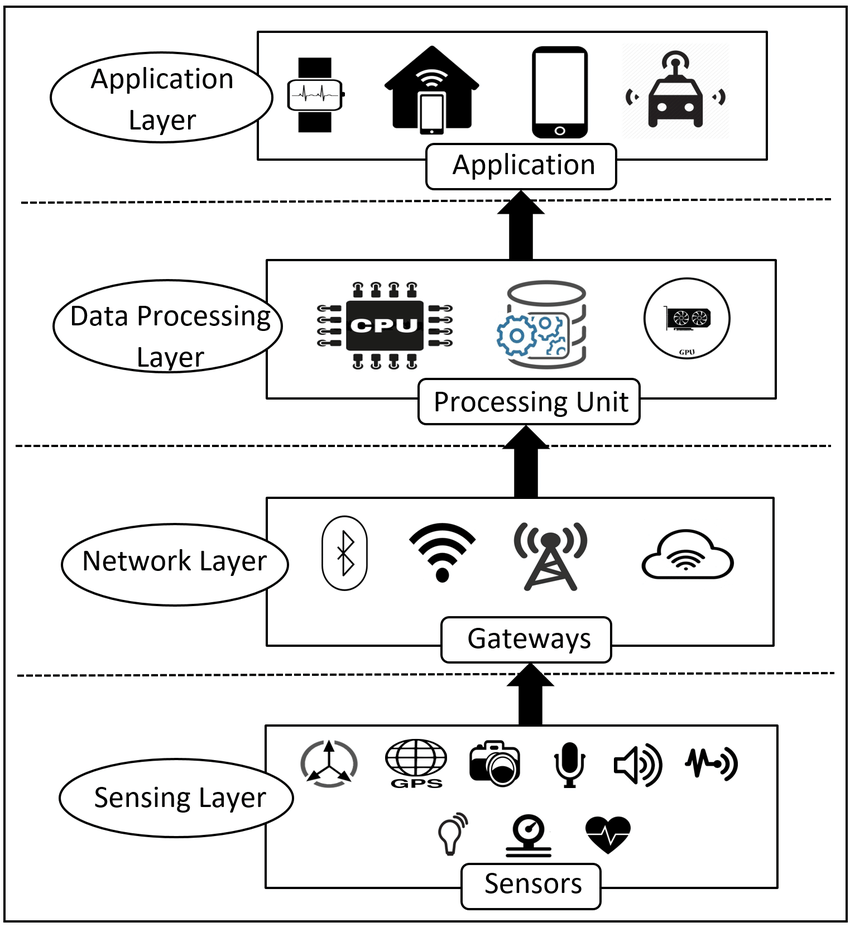
\includegraphics[width=0.7\linewidth]{figures/IoT-Architecture-Layers-and-Components.png}
%  \caption{Diagrama general de un sistema IoT}
%  \label{fig:IoT_General}
%\end{figure}


\section{Contexto tecnológico}

Esta sección recoge la información relativa a las tecnologías y herramientas más relevantes dentro del contexto del desarrollo de este proyecto.


\chapter{Estado del arte}
\label{chapter:estado_arte}

\chapquote{La ciencia amigo, está compuesta de errores; pero son errores que es útil cometer ya que nos acercan poco a poco hacia la verdad.}{Julio Verne}


En este capítulo se introduce una revisión del estado del arte y del estado de la cuestión en lo que respecta al marco teórico del proyecto que se propone en este TFM, así como una descripción sobre los sistemas que existen en el mercado o que han sido reportados en la literatura, los cuales presentan aspectos comunes con la solución propuesta.
%\section{Energías renovables: ¿Qué son?}


\section{Análisis de la situación actual}

En esta sección, se pone en valor y/o contraste la información introducida en las secciones anteriores, de tal forma que pueda realizarse un análisis del entorno en el que se desarrolla este proyecto, así como también se pueda poner de manifiesto la relevancia y la idoneidad del desarrollo propuesto. 


\todo[inline]{Aqui si hay que introducir los wearbles}

\subsection{Proyectos relacionados}

Tenemos aqui el proyecto DemonicSalmon de 2018 de 72 universitarios entre 18 y 23 años. Datos no wearables: movilidad (que mejor la de la pulsera), actividad (aqui igual), patrones de comunicación.

Student life es el mitico de 2014, el de las 10 semanas con cuestionarios. Aqui usaban datos como micro, sensor de luz, gps, bluetooth y acelerometro para determinar actividad, conversacion,sueño y localizacion.

Sus cuestionarios de contraste con PSS, PHQ9 y UCLA pero solo ANTES y DESPUES de acabar el estudio, no diarios. Tirar con las correlaciones desde aqui.

El paper de Smart Devices andWearable Technologies to Detect and
Monitor Mental Health Conditions and Stress:
A Systematic Review sirve para ver que datos valen para algo: variabilidad del ritmo cardiaco,  electroencefalograma (nope). Mirar los resultados para eso. Es de 2021.

Dataset wesad, 2018 alemania, pero si son invasivos. Ahi tiramos la trama para desmarcarnos de eso. Lo mismo con PASS, diciembre 2020 pero también pilla ritmo caridaco.

\subsection{Contribución de la solución propuesta}

Usamos datos de wearables compatibles con varios fabricantes.
Cuestionarios diarios además de los de 12 semanas, tanto mañana y noche.
\chapter{Metodología}
\label{chapter:metodologia}

En este capítulo, se introducen algunas de las principales metodologías de desarrollo \textit{software} que actualmente más se utilizan.

\section{Metodologías de desarrollo del \textit{software} de Sistemas}

\subsection*{Metodología del desarrollo seleccionada}


\chapter{Análisis del sistema propuesto}
\label{chapter:analisis}

\chapquote{Cada día me gusta levantarme porque hay otro reto.}{Roger Penske}

El propósito de este capítulo consiste en la \gls{ers} correspondiente al proyecto desarrollado en este \gls{tfm}. Para la elaboración de la misma se ha tomado como base el estándar IEEE 830 \cite{noauthor_ieee_1998}.

Esta especificación recoge todas las características, objetivos, restricciones y suposiciones para el desarrollo del proyecto, definiendo claramente el sistema a desarrollar y sirviendo asimismo de referencia para la verificación y validación de la solución implementada. Para dicha definición en primer lugar serán documentadas qué restricciones, suposiciones y dependencias son asumidas para posteriormente determinar los requisitos de usuario, los requisitos no funcionales y por último, los requisitos de interfaces externas.

Por otra parte, dado que este proyecto tiene una naturaleza abierta y transparente, en especial al tratar datos sensibles; el público objetivo de esta especificación de requisitos es cualquier persona que desee conocer las características del sistema y sobre qué criterios, restricciones o supuestos ha sido diseñado, incrementando la confianza social en el proyecto.
        
\section{Alcance}
    \label{req:intro:alcance}
    Como ya se mencionó en la Sección \ref{sec:objetivos}, el objetivo principal de este \gls{tfm} es la creación de un prototipo de un sistema que permita la detección precoz y la mejora de los trastornos de salud mental en la comunidad universitaria. 

    Este proyecto se fundamenta en la alarmante situación psicológica que atraviesa nuestra sociedad, partiendo de la premisa de que en numerosas ocasiones las personas desconocen factores, conductas o síntomas relacionados con problemas de salud mental, pero que mejorando la conciencia de los mismos se podría reducir el número y la gravedad de los casos.

    Para ello, este sistema se encargará de monitorizar y visualizar las medidas de estrés, soledad, depresión y suicidio, en base a cuestionarios que la persona rellene diariamente; planteándose un complemento para mejorar la sensibilidad de los usuarios sobre la evolución de su salud mental. Para ello, aportará consejos y remitiendo a un profesional cuando la situación del usuario sea delicada; quedando fuera del proyecto cuestiones como el asesoramiento médico profesional o una atención psicológica personalizada.

    Dichos consejos estarán personalizados para el nivel de gravedad (o ausencia de la misma) de cada medida permitiendo además, que el usuario pueda ver claramente cómo se ha sentido durante los últimos días, semanas o meses para cada variable.

    Por otra parte, para reducir la estigmatización que aún hoy se percibe de la Salud Mental, el sistema presentará al usuario una visualización de una serie de datos sobre estrés, soledad y depresión del resto de usuarios.

    Asimismo, la aplicación recopilará los datos de su dispositivo \gls{wearable} a los que el usuario haya dado acceso con la finalidad de construir un conjunto de datos anonimizado con el que se pueda desarrollar un modelo predictivo de esas medidas, permitiendo un apoyo más integral al usuario. 

    Finalmente, tanto la información de los datos de las medidas del usuario como sus datos sanitarios, serán enviados a un servidor alojado en la universidad para su guardado únicamente en el caso de los datos sanitarios. En cuanto a las medidas de los usuarios, serán guardadas y procesadas para presentar al usuario las tendencias del resto de usuarios.
    
    La \gls{ers} que se presenta a continuación se estructura de la siguiente forma:

    \begin{enumerate}
        \item En la Sección \ref{req:descripcion} se especifica la descripción general del producto a desarrollar. Para ello, se pone al usuario en contexto (Sección \ref{req:descripcion:perspectiva}), para continuar especificando los usuarios del producto (Sección \ref{req:descripcion:usuarios}). Tras ello se detallarán las restricciones generales del producto, sus suposiciones y dependencias en las secciones 
        \ref{req:descripcion:restricciones}, \ref{req:descripcion:suposiciones} y \ref{req:descripcion:dependencias}, respectivamente.
        \item Posteriormente, en la Sección \ref{req:especificos} se detalla la especificación formal de los requisitos del proyecto propiamente dicha. En la Sección \ref{req:especificos:funcionales} se definirán los requisitos de los usuarios finales que especifican las necesidades de los mismos. Cada requisito de usuario será descompuesto en uno o más requisitos funcionales, mientras que los no funcionales estarán desglosados por categorías en la Sección \ref{req:especificos:no_funcionales}.
        \item Por último, en la Sección \ref{req:externas} se detallarán los requisitos de interfaces hardware y software que caracterizan las conexiones entre componentes (Secciones \ref{req:externas:hardware} y \ref{req:externas:software}, respectivamente), y las restricciones de desarrollo en la Sección \ref{req:externas:restricciones}.
    \end{enumerate}
    
\section{Descripción general del producto}
    \label{req:descripcion}

    \subsection{Perspectiva del producto}
        \label{req:descripcion:perspectiva}

        Como se detalló en las secciones \ref{sec:objetivos} y \ref{req:intro:alcance}, el objetivo principal de este \gls{tfm} es la creación de un prototipo de un Sistema para el Bienestar Emocional, sobre el cual pueda servir como punto de partida para proyectos de futuros alumnos, incorporando más funcionalidades y profundidad en las mismas sin necesidad de rehacer gran parte del trabajo. 

        Este prototipo, a través de su aplicación móvil, se apoyará en el sistema operativo Android para su posible uso en una enorme variedad de dispositivos móviles. Asimismo, a través de su \gls{sdk}, se interactuará con el sistema operativo para ciertos escenarios, como la planificación de tareas.

        Por otra parte, para la lectura de datos de los \glspl{wearable} se contará con en el nuevo componente de Android \textit{Salud Conectada} (o \textit{Health Connect} en inglés). Dicho componente permitirá la abstracción de los componentes hardware delegando a los fabricantes la conexión de sus dispositivos con este sistema y unificando el acceso y uso de los datos de actividad física. La extracción de datos por otros canales queda fuera de este proyecto, ya que los cauces legales están fuertemente restringidos. 

        En cuanto al procesamiento de los datos será utilizado un servidor puesto a disposición por la Universidad como prototipo, no contemplándose ningún trabajo de despliegue en un escenario real del mismo.

        Asimismo, para el diseño de las medidas de seguimiento y los consejos para los usuarios se ha contado con la colaboración de dos psicólogas investigadoras, las cuales han asesorado en la elección de los cuestionarios puntuales y han elaborado el contenido tanto de los cuestionarios diarios como de las recomendaciones. 
        
        Por último, se busca que este sistema sea un marco para la investigación en el campo de la Psicología permitiendo la realización de experimentos que necesiten acceso a datos de actividad física o cuestionarios.


    \subsection{Características de los usuarios finales}
        \label{req:descripcion:usuarios}
        
        Los usuarios finales de este sistema serán los miembros de la comunidad universitaria que deseen monitorizar su salud mental, sin necesidad de conocimientos específicos. No obstante, deberán de cumplir con las siguientes pautas:
    
        \begin{enumerate}
            \item Los usuarios dispondrán de un \gls{smartphone} con sistema operativo Android, cuya versión cumpla la \ref{req:restriccion:android_minimo}.
            \item El usuario realizará de forma habitual los cuestionarios ofrecidos por la aplicación.
            \item El usuario estará dispuesto a que sus respuestas a los cuestionarios sean subidas a un servidor de la universidad, con un identificador de usuario anónimo.
            \item Opcionalmente, el usuario dispondrá de un dispositivo \gls{wearable} compatible con \textit{Salud Conectada}, con la aplicación del fabricante\footnote{A fecha de realización de este proyecto, los fabricantes que garantizan compatibilidad con este ecosistema son Fitbit o Samsung} correspondiente instalada y el dispositivo conectado a su \gls{smartphone}.
            
        \end{enumerate}
        
    \subsection{Restricciones generales}
        \label{req:descripcion:restricciones}
        Debido funcionalmente a los componentes en los que se apoya el proyecto para ser implementable, es necesario definir ciertas restricciones generales, a saber:
        \begin{enumerate}[label=\textbf{RG-\arabic*}]
            \item \label{req:restriccion:android_referencia} La aplicación se ejecutará sobre el sistema operativo Android. Concretamente, se tomará Android 14 como referencia.
            \item \label{req:restriccion:android_minimo} La aplicación especificará Android 9 como versión mínima, pudiéndose ejecutar la aplicación en cualquier versión entre la mínima y la referente.
        \end{enumerate}
    
    \subsection{Suposiciones}
        \label{req:descripcion:suposiciones}

        \begin{enumerate}[label=\textbf{SUP-\arabic*}]
            \item El usuario de la aplicación dispone de conexión a Internet de forma habitual.
            \item El usuario de la aplicación es el mismo que utiliza el dispositivo \gls{wearable}.
            \item Las respuestas del usuario a los cuestionarios serán veraces y verídicas.
            \item El usuario rellenará frecuentemente los cuestionarios.
            \item El usuario utilizará con cierta asiduidad el dispositivo \gls{wearable}.
            \item El servidor donde se aloja el componente homónimo está disponible.
            \item El usuario desactiva el ahorro de batería relativo a la aplicación, para que la optimización de energía del sistema operativo no interfiera con la aplicación en determinados escenarios.
            \item Se supone que habrá más de un usuario utilizando la aplicación diariamente.
            \item Se supone que el dispositivo móvil que ejecute la aplicación es un \gls{smartphone} o una tableta, no otros dispositivos Android como televisores o bajo emulación, los cuales teóricamente podrían ejecutar la aplicación.
        \end{enumerate}
        
    \subsection{Dependencias}
        \label{req:descripcion:dependencias}
    
        \begin{enumerate}[label=\textbf{DEP-\arabic*}]
            \item \label{req:dependencias:integracion_correcta} Para garantizar la lectura de los datos del dispositivo \gls{wearable}, el fabricante debe integrar su sistema con el \gls{framework} de \textit{Salud Conectada}, escribiendo regularmente en este componente los datos recogidos por el \gls{wearable}.
            \item En relación con \ref{req:dependencias:integracion_correcta}, el \gls{wearable} del usuario escribirá en \textit{Salud Conectada} los datos recogidos.
            \item \label{req:dependencias:planificacion} Para la ejecución de las tareas recurrentes es necesario que el sistema operativo otorgue recursos de ejecución a la aplicación.
        \end{enumerate}

\section{Requisitos específicos}
    \label{req:especificos}

    \subsection{Requisitos funcionales}
        \label{req:especificos:funcionales}

        Siguiendo las pautas de algunas metodologías tradicionales o híbridas dentro de la Ingeniería de Requisitos, aquellas que, como por ejemplo tienen descritas sus prácticas en el libro \textit{Software Requirements} \cite{wiegers_software_2013}, en esta sección de se definirán los requisitos funcionales del sistema a desarrollar agrupados por sus correspondientes requisitos de usuario. En este contexto, los requisitos de usuario tiene como finalidad describir las necesidades de usuario de las que se derivan dichos requisitos funcionales. 

        \newlist{req-usuario}{enumerate}{1}
        \newlist{req-funcionales}{enumerate}{1}

        \begin{enumerate}[series=req-usuario,label=\textbf{\texttt{RU-\arabic*}}]
            \item \label{req:usuario:seguimiento_estres} Como usuario, quiero realizar un seguimiento del estrés para controlar mi evolución del mismo.
            \begin{enumerate}[series=req-funcionales,label=\textbf{\texttt{RF-\arabic*}}]
                \item \label{req:funcionales:estres_diario_info} El seguimiento del estrés se realizará mediante cuestionarios diarios que recogerán la siguiente información del usuario: nerviosismo, angustia, sensación de actividad y preocupación.
                \item \label{req:funcionales:estres_diario_manana} La aplicación desplegará un cuestionario matutino diario de estrés sobre las 9:00 hora local del usuario, recogiendo la siguiente información del nerviosismo, angustia, sensación de actividad y preocupación relativa al momento correspondiente. La definición de este cuestionario se recoge en el Anexo \ref{cuestionarios:estres_manana}.
                \item \label{req:funcionales:estres_diario_noche}  La aplicación desplegará un cuestionario vespertino diario de estrés sobre las 21:00 hora local del usuario, recogiendo la siguiente información del nerviosismo, angustia, sensación de actividad y preocupación relativa al día en su totalidad. La definición de este cuestionario se recoge en el Anexo \ref{cuestionarios:estres_noche}.
                \item \label{req:funcionales:estres_puntual} La aplicación desplegará un cuestionario puntual para el seguimiento del estrés sobre las 15:00 hora local del usuario, cada dos semanas. Dicho cuestionario será el PSS-10, cuya definición se recoge en el Anexo \ref{cuestionarios:pss_10}.
                \item \label{req:funcionales:estres_umbrales} La medida estrés estará calibrada en tres umbrales, a saber: baja, moderada y alta.
                \item \label{req:funcionales:estres_umbrales_consejo} Para cada umbral de la medida de estrés se dispondrá de al menos un mensaje o recomendación.
                \item \label{req:funcionales:estres_notificacion} La creación de cada cuestionario de estrés será notificada al usuario.
                \item \label{req:funcionales:estres_cuestionario_aplazar} La aplicación permitirá ir guardando parcialmente las respuestas que un usuario realice de un cuestionario de estrés.
                \item \label{req:funcionales:estres_cuestionario_pendientes} La aplicación mostrará al usuario si dispone de cuestionarios de estrés por completar para su finalización.
                \item \label{req:funcionales:estres_cuestionario_numero} Al finalizar un cuestionario de estrés, se le presentará al usuario el resultado numérico del mismo.
                \item \label{req:funcionales:estres_cuestionario_categoria} Al finalizar un cuestionario de estrés, se le presentará al usuario el resultado cualitativo del mismo.
                \item \label{req:funcionales:estres_cuestionario_consejo} Al finalizar un cuestionario de estrés, se le presentará al usuario un consejo o recomendación según su nivel de estrés.
            \end{enumerate}
        \end{enumerate}
        \begin{enumerate}[resume=req-usuario,label=\textbf{\texttt{RU-\arabic*}}]
            \item \label{req:usuario:seguimiento_depresion} Como usuario quiero realizar un seguimiento de la depresión para controlar mis niveles de la misma.
            \begin{enumerate}[resume=req-funcionales,label=\textbf{\texttt{RF-\arabic*}}]
                \item \label{req:funcionales:depresion_diario_info} El seguimiento de la depresión se realizará mediante cuestionarios diarios que recogerán la siguiente información del usuario: tristeza, apatía y sensación de vacío.
                \item \label{req:funcionales:depresion_diario_manana} La aplicación desplegará un cuestionario matutino diario de depresión sobre las 9:00, hora local del usuario, recogiendo la siguiente información de la tristeza, apatía y sensación de vacío relativa al momento correspondiente. La definición de este cuestionario se recoge en el Anexo \ref{cuestionarios:depresion_manana}.
                \item \label{req:funcionales:depresion_diario_noche}  La aplicación desplegará un cuestionario vespertino diario de depresión sobre las 21:00, hora local del usuario, recogiendo la siguiente información de la tristeza, apatía y sensación de vacío relativa al día en su totalidad. La definición de este cuestionario se recoge en el Anexo \ref{cuestionarios:depresion_noche}.
                \item \label{req:funcionales:depresion_puntual} La aplicación desplegará un cuestionario puntual para el seguimiento de la depresión sobre las 15:00, hora local del usuario, cada dos semanas. Dicho cuestionario será el PHQ-9, cuya definición se recoge en el Anexo \ref{cuestionarios:phq_9}.
                \item \label{req:funcionales:depresion_umbrales} La medida depresión estará calibrada en tres umbrales, a saber: baja, moderada y alta.
                \item \label{req:funcionales:depresion_umbrales_consejo} Para cada umbral de la medida depresión se dispondrá de al menos un mensaje o recomendación.
                \item \label{req:funcionales:depresion_notificacion} La creación de cada cuestionario de depresión será notificada al usuario.
                \item \label{req:funcionales:depresion_cuestionario_aplazar} La aplicación permitirá ir guardando parcialmente las respuestas que un usuario realice de un cuestionario de depresión.
                \item \label{req:funcionales:depresion_cuestionario_pendientes} La aplicación mostrará al usuario si dispone de cuestionarios de depresión por completar.
                \item \label{req:funcionales:depresion_cuestionario_numero} Al finalizar un cuestionario de depresión, se le presentará al usuario el resultado numérico del mismo.
                \item \label{req:funcionales:depresion_cuestionario_categoria} Al finalizar un cuestionario de depresión, se le presentará al usuario el resultado cualitativo del mismo.
                \item \label{req:funcionales:depresion_cuestionario_consejo} Al finalizar un cuestionario de depresión, se le presentará al usuario un consejo o recomendación según su nivel de depresión.
            \end{enumerate}
        \end{enumerate}
        \begin{enumerate}[resume=req-usuario,label=\textbf{\texttt{RU-\arabic*}}]
            \item \label{req:usuario:seguimiento_soledad} Como usuario, quiero realizar un seguimiento de la soledad para controlar mis niveles de la misma.
            \begin{enumerate}[resume=req-funcionales,label=\textbf{\texttt{RF-\arabic*}}]
                \item \label{req:funcionales:soledad_diario_info} El seguimiento de la soledad se realizará mediante cuestionarios diarios que recogerán la siguiente información del usuario: sensación de soledad, sentimiento de incomprensión y sensación de falta de apoyo.
                \item \label{req:funcionales:soledad_diario_manana} La aplicación desplegará un cuestionario matutino diario de soledad sobre las 9:00, hora local del usuario, recogiendo la siguiente información de la sensación de soledad, sentimiento de incomprensión y sensación de falta de apoyo relativa al momento correspondiente. La definición de este cuestionario se recoge en el Anexo \ref{cuestionarios:soledad_manana}.
                \item \label{req:funcionales:soledad_diario_noche}  La aplicación desplegará un cuestionario vespertino diario de soledad sobre las 21:00, hora local del usuario, recogiendo la siguiente información de la sensación de soledad, sentimiento de incomprensión y sensación de falta de apoyo relativa al día en su totalidad. La definición de este cuestionario se recoge en el Anexo \ref{cuestionarios:soledad_noche}.
                \item \label{req:funcionales:soledad_puntual} La aplicación desplegará un cuestionario puntual para el seguimiento de la soledad sobre las 15:00, hora local del usuario, cada dos semanas. Dicho cuestionario será el UCLA-20, cuya definición se recoge en el Anexo \ref{cuestionarios:ucla_20}.
                \item \label{req:funcionales:soledad_umbrales} La medida soledad estará calibrada en tres umbrales, a saber: baja, moderada y alta.
                \item \label{req:funcionales:soledad_umbrales_consejo} Para cada umbral de la medida soledad se dispondrá de al menos un mensaje o recomendación.
                \item \label{req:funcionales:soledad_notificacion} La creación de cada cuestionario de soledad será notificada al usuario.
                \item \label{req:funcionales:soledad_cuestionario_aplazar} La aplicación permitirá ir guardando parcialmente las respuestas que un usuario realice de un cuestionario de soledad.
                \item \label{req:funcionales:soledad_cuestionario_pendientes} La aplicación mostrará al usuario si dispone de cuestionarios de soledad por completar para su finalización.
                \item \label{req:funcionales:soledad_cuestionario_numero} Al finalizar un cuestionario de soledad, se le presentará al usuario el resultado numérico del mismo.
                \item \label{req:funcionales:soledad_cuestionario_categoria} Al finalizar un cuestionario de soledad, se le presentará al usuario el resultado cualitativo del mismo.
                \item \label{req:funcionales:soledad_cuestionario_consejo} Al finalizar un cuestionario de soledad, se le presentará al usuario un consejo o recomendación según su nivel de soledad.
            \end{enumerate}
        \end{enumerate}
        \begin{enumerate}[resume=req-usuario,label=\textbf{\texttt{RU-\arabic*}}]
            \item \label{req:usuario:seguimiento_suicidio}  Como usuario, quiero realizar un seguimiento del riesgo de suicidio para controlar mi nivel del mismo.
            \begin{enumerate}[resume=req-funcionales,label=\textbf{\texttt{RF-\arabic*}}]
                \item \label{req:funcionales:suicidio_diario_info} El seguimiento del riesgo de suicidio se realizará mediante cuestionarios diarios que recogerán la siguiente información del usuario: pensamientos suicidas y posibilidades de suicidio.
                \item \label{req:funcionales:suicidio_diario_manana} La aplicación desplegará un cuestionario matutino diario de riesgo de suicidio sobre las 9:00, hora local del usuario, recogiendo la siguiente información de los pensamientos suicidas y posibilidades de suicidio relativa al momento correspondiente. La definición de este cuestionario se recoge en el Anexo \ref{cuestionarios:suicidio_manana}.
                \item \label{req:funcionales:suicidio_diario_noche}  La aplicación desplegará un cuestionario vespertino diario de riesgo de suicidio sobre las 21:00, hora local del usuario, recogiendo la siguiente información de los pensamientos suicidas y posibilidades de suicidio relativa al día en su totalidad. La definición de este cuestionario se recoge en el Anexo \ref{cuestionarios:suicidio_noche}.
                \item \label{req:funcionales:suicidio_umbrales} La medida de riesgo de suicidio estará calibrada en tres umbrales, a saber: bajo, moderado y alto.
                \item \label{req:funcionales:suicidio_consejo} Para cada umbral de la medida riesgo de suicidio se dispondrá de al menos un mensaje o recomendación.
                \item \label{req:funcionales:suicidio_notificacion} La creación de cada cuestionario de riesgo de suicidio será notificada al usuario.
                \item \label{req:funcionales:suicidio_cuestionario_aplazar} La aplicación permitirá ir guardando parcialmente las respuestas que un usuario realice de un cuestionario de suicidio.
                \item \label{req:funcionales:suicidio_cuestionario_pendientes} La aplicación mostrará al usuario si dispone de cuestionarios de riesgo de suicidio por completar.
                \item \label{req:funcionales:suicidio_cuestionario_consejo} Al finalizar un cuestionario de riesgo de suicidio, se le presentará al usuario un consejo o recomendación según su nivel de riesgo de suicidio.
            \end{enumerate}
        \end{enumerate}
        \begin{enumerate}[resume=req-usuario,label=\textbf{\texttt{RU-\arabic*}}]
            \item \label{req:usuario:visualizar_estres} Como usuario, quiero visualizar mi nivel más reciente de estrés de forma fácil para que pueda tomar conciencia de mi estado y recordarlo.
            \begin{enumerate}[resume=req-funcionales,label=\textbf{\texttt{RF-\arabic*}}]
                \item \label{req:funcionales:visualizar_estres_numero} La aplicación mostrará al usuario el resultado numérico del último cuestionario de estrés.
                \item \label{req:funcionales:visualizar_estres_categoria} La aplicación mostrará al usuario el nivel cualitativo del último cuestionario de estrés.
            \end{enumerate}
        \end{enumerate}
        \begin{enumerate}[resume=req-usuario,label=\textbf{\texttt{RU-\arabic*}}]
            \item \label{req:usuario:visualizar_depresion} Como usuario, quiero visualizar mi nivel más reciente de la depresión de forma fácil para que pueda tomar conciencia de mi estado y recordarlo.
            
            \begin{enumerate}[resume=req-funcionales,label=\textbf{\texttt{RF-\arabic*}}]
                \item \label{req:funcionales:visualizar_depresion_numero} La aplicación mostrará al usuario el resultado numérico del último cuestionario de depresión.
                \item \label{req:funcionales:visualizar_depresion_categoria} La aplicación mostrará al usuario el nivel cualitativo del último cuestionario de depresión.
            \end{enumerate}
        \end{enumerate}
        \begin{enumerate}[resume=req-usuario,label=\textbf{\texttt{RU-\arabic*}}]
            \item \label{req:usuario:visualizar_soledad} Como usuario, quiero visualizar mi nivel más reciente de soledad de forma fácil para que pueda tomar conciencia de mi estado y recordarlo.
            \begin{enumerate}[resume=req-funcionales,label=\textbf{\texttt{RF-\arabic*}}]
                \item \label{req:funcionales:visualizar_soledad_numero} La aplicación mostrará al usuario el resultado numérico del último cuestionario de soledad.
                \item \label{req:funcionales:visualizar_soledad_categoria} La aplicación mostrará al usuario el nivel cualitativo del último cuestionario de soledad.
            \end{enumerate}
        \end{enumerate}
        \begin{enumerate}[resume=req-usuario,label=\textbf{\texttt{RU-\arabic*}}]
            \item \label{req:usuario:consejo_estres} Como usuario, quiero disponer de al menos un consejo para cada nivel de estrés para saber cómo reducirlo en cada momento.
            \begin{enumerate}[resume=req-funcionales,label=\textbf{\texttt{RF-\arabic*}}]
                \item \label{req:funcionales:consejo_cuestionario_estres} La aplicación mostrará un consejo sobre el nivel de estrés registrado al terminar un cuestionario.
                \item \label{req:funcionales:consejo_visualizacion_estres} En la visualización de la última medición de estrés se podrá consultar un consejo sobre el mismo. 
            \end{enumerate}
        \end{enumerate}
        \begin{enumerate}[resume=req-usuario,label=\textbf{\texttt{RU-\arabic*}}]
            \item \label{req:usuario:consejo_depresion} Como usuario, quiero disponer de al menos un consejo para cada nivel de depresión para saber cómo reducirlo en cada momento.
            \begin{enumerate}[resume=req-funcionales,label=\textbf{\texttt{RF-\arabic*}}]
                \item \label{req:funcionales:consejo_cuestionario_depresion} La aplicación mostrará un consejo sobre el nivel de depresión registrado al terminar un cuestionario.
                \item \label{req:funcionales:consejo_visualizacion_depresion} En la visualización de la última medición de depresión se podrá consultar un consejo sobre el mismo.
            \end{enumerate}
        \end{enumerate}
        \begin{enumerate}[resume=req-usuario,label=\textbf{\texttt{RU-\arabic*}}]
            \item \label{req:usuario:consejo_soledad} Como usuario, quiero disponer de al menos un consejo para cada nivel de soledad para saber cómo reducirlo en cada momento.
            \begin{enumerate}[resume=req-funcionales,label=\textbf{\texttt{RF-\arabic*}}]
                \item \label{req:funcionales:consejo_cuestionario_soledad} La aplicación mostrará un consejo sobre el nivel de soledad registrado al terminar un cuestionario.
                \item \label{req:funcionales:consejo_visualizacion_soledad} En la visualización de la última medición de soledad se podrá consultar un consejo sobre el mismo. 
            \end{enumerate}
        \end{enumerate}
        \begin{enumerate}[resume=req-usuario,label=\textbf{\texttt{RU-\arabic*}}]
            \item \label{req:usuario:consejo_suicidio} Como usuario, quiero disponer de al menos un consejo para cada nivel de riesgo de suicidio para saber cómo reducirlo en cada momento.
            \begin{enumerate}[resume=req-funcionales,label=\textbf{\texttt{RF-\arabic*}}]
                \item \label{req:funcionales:consejo_cuestionario_suicidio} La aplicación mostrará un consejo sobre el nivel de riesgo de suicidio registrado al terminar un cuestionario.
            \end{enumerate}
        \end{enumerate}
        \begin{enumerate}[resume=req-usuario,label=\textbf{\texttt{RU-\arabic*}}]
            \item \label{req:usuario:evolucion_estres}  Como usuario, quiero visualizar la evolución de mis registros de estrés para observarla a lo largo del tiempo.
            \begin{enumerate}[resume=req-funcionales,label=\textbf{\texttt{RF-\arabic*}}]
                \item \label{req:funcionales:evolucion_estres_dia} El usuario podrá visualizar sus estadísticas de estrés agrupadas por día.
                \item \label{req:funcionales:evolucion_estres_semana} El usuario podrá visualizar sus estadísticas de estrés agrupadas por semana.
                \item \label{req:funcionales:evolucion_estres_mes} El usuario podrá visualizar sus estadísticas de estrés agrupadas por mes.
                \item \label{req:funcionales:evolucion_estres_elegir} El usuario podrá escoger el intervalo de tiempo sobre el cual desea consultar sus estadísticas de estrés.
            \end{enumerate}
        \end{enumerate}
        \begin{enumerate}[resume=req-usuario,label=\textbf{\texttt{RU-\arabic*}}]
            \item \label{req:usuario:evolucion_depresion} Como usuario, quiero visualizar la evolución de mis registros de depresión para observarla a lo largo del tiempo.
            \begin{enumerate}[resume=req-funcionales,label=\textbf{\texttt{RF-\arabic*}}]
                \item \label{req:funcionales:evolucion_depresion_dia} El usuario podrá visualizar sus estadísticas de depresión agrupadas por día.
                \item \label{req:funcionales:evolucion_depresion_semana} El usuario podrá visualizar sus estadísticas de depresión agrupadas por semana.
                \item \label{req:funcionales:evolucion_depresion_mes} El usuario podrá visualizar sus estadísticas de depresión agrupadas por mes.
                \item \label{req:funcionales:evolucion_depresion_elegir} El usuario podrá escoger el intervalo de tiempo sobre el cual desea consultar sus estadísticas de depresión.
            \end{enumerate}
        \end{enumerate}
        \begin{enumerate}[resume=req-usuario,label=\textbf{\texttt{RU-\arabic*}}]
            \item \label{req:usuario:evolucion_soledad} Como usuario, quiero visualizar la evolución de mis registros de soledad para observarla a lo largo del tiempo.
            \begin{enumerate}[resume=req-funcionales,label=\textbf{\texttt{RF-\arabic*}}]
                \item \label{req:funcionales:evolucion_soledad_dia} El usuario podrá visualizar sus estadísticas de soledad agrupadas por día.
                \item \label{req:funcionales:evolucion_soledad_semana} El usuario podrá visualizar sus estadísticas de soledad agrupadas por semana.
                \item \label{req:funcionales:evolucion_soledad_mes} El usuario podrá visualizar sus estadísticas de soledad agrupadas por mes.
                \item \label{req:funcionales:evolucion_soledad_elegir} El usuario podrá escoger el intervalo de tiempo sobre el cual desea consultar sus estadísticas de soledad.
            \end{enumerate}
        \end{enumerate}
        \begin{enumerate}[resume=req-usuario,label=\textbf{\texttt{RU-\arabic*}}]
            \item \label{req:usuario:comunidad_estres} Como usuario, deseo consultar estadísticas de estrés de la comunidad de usuarios para poner en contexto mis niveles y apreciar la evolución de la comunidad.
            \begin{enumerate}[resume=req-funcionales,label=\textbf{\texttt{RF-\arabic*}}]
                \item \label{req:funcionales:comunidad_estres_dia_anterior_ver} El usuario podrá visualizar la media de estrés que han exhibido los usuarios de la comunidad durante el día anterior.
                \item \label{req:funcionales:comunidad_estres_siete_dias_ver} El usuario podrá visualizar la media de estrés de los usuarios de la comunidad que se ha observado en los últimos siete días.
                \item \label{req:funcionales:comunidad_estres_semana_actual_ver} El usuario podrá visualizar la media de estrés de los usuarios de la comunidad sobre los datos de la semana actual.
            \end{enumerate}
        \end{enumerate}
        \begin{enumerate}[resume=req-usuario,label=\textbf{\texttt{RU-\arabic*}}]
            \item \label{req:usuario:comunidad_depresion} Como usuario, deseo consultar estadísticas de depresión de la comunidad de usuarios para poner en contexto mis niveles y apreciar la evolución de la comunidad.
            \begin{enumerate}[resume=req-funcionales,label=\textbf{\texttt{RF-\arabic*}}]
                \item \label{req:funcionales:comunidad_depresion_dia_anterior_ver} El usuario podrá visualizar la media de depresión que han exhibido los usuarios de la comunidad durante el día anterior.
                \item \label{req:funcionales:comunidad_depresion_siete_dias_ver} El usuario podrá visualizar la media de depresión de los usuarios de la comunidad que se ha observado en los últimos siete días.
                \item \label{req:funcionales:comunidad_depresion_semana_actual_ver} El usuario podrá visualizar la media de depresión de los usuarios de la comunidad sobre los datos de la semana actual.
            \end{enumerate}
        \end{enumerate}
        \begin{enumerate}[resume=req-usuario,label=\textbf{\texttt{RU-\arabic*}}]
            \item \label{req:usuario:comunidad_soledad}  Como usuario, deseo consultar estadísticas de soledad de la comunidad de usuarios para poner en contexto mis niveles y apreciar la evolución de la comunidad.
            \begin{enumerate}[resume=req-funcionales,label=\textbf{\texttt{RF-\arabic*}}]
                \item \label{req:funcionales:comunidad_soledad_dia_anterior_ver} El usuario podrá visualizar la media de soledad que han exhibido los usuarios de la comunidad durante el día anterior.
                \item \label{req:funcionales:comunidad_soledad_siete_dias_ver} El usuario podrá visualizar la media de soledad de los usuarios de la comunidad que se ha observado en los últimos siete días.
                \item \label{req:funcionales:comunidad_soledad_semana_actual_ver} El usuario podrá visualizar la media de soledad de los usuarios de la comunidad sobre los datos de la semana actual.
            \end{enumerate}
        \end{enumerate}
            
        \begin{enumerate}[resume=req-usuario,label=\textbf{\texttt{RU-\arabic*}}]
            \item \label{req:usuario:visualizar_actividad_fisica} Como usuario, quiero visualizar mis datos de actividad física recogidos por la aplicación.
            \begin{enumerate}[resume=req-funcionales,label=\textbf{\texttt{RF-\arabic*}}]
                \item \label{req:funcionales:permiso_distancia} La aplicación solicitará al usuario explícitamente el permiso de lectura de los datos de la distancia recorrida recogidos desde el dispositivo \gls{wearable}.
                \item \label{req:funcionales:permiso_desnivel} La aplicación solicitará al usuario explícitamente el permiso de lectura de los datos del desnivel obtenido recogidos desde el dispositivo \gls{wearable}. 
                \item \label{req:funcionales:permiso_ejercicio} La aplicación solicitará al usuario explícitamente el permiso de lectura de los datos de las sesiones de ejercicio realizadas recogidos desde el dispositivo \gls{wearable}.
                \item \label{req:funcionales:permiso_plantas} La aplicación solicitará al usuario explícitamente el permiso de lectura de los datos de los pisos subidos durante la actividad física recogidos desde el dispositivo \gls{wearable}.
                \item \label{req:funcionales:permiso_pulsaciones} La aplicación solicitará al usuario explícitamente el permiso de lectura de los datos de la frecuencia cardíaca recogidos desde el dispositivo \gls{wearable}.
                \item \label{req:funcionales:permiso_sueno} La aplicación solicitará al usuario explícitamente el permiso de lectura de los datos de sueño recogidos desde el dispositivo \gls{wearable}.
                \item \label{req:funcionales:permiso_pasos} La aplicación solicitará al usuario explícitamente el permiso de lectura de los datos de los pasos realizados recogidos desde el dispositivo \gls{wearable}.
                \item \label{req:funcionales:permiso_calorias} La aplicación solicitará al usuario explícitamente el permiso de lectura de los datos de las calorías quemadas recogidos desde el dispositivo \gls{wearable}.
                \item \label{req:funcionales:permiso_peso} La aplicación solicitará al usuario explícitamente el permiso de lectura de los datos del peso corporal recogidos desde el dispositivo \gls{wearable}.
                \item \label{req:funcionales:extraer_distancia} La aplicación extraerá del dispositivo \gls{wearable} los datos de la distancia recorrida por el usuario.
                \item \label{req:funcionales:extraer_desnivel} La aplicación extraerá del dispositivo \gls{wearable} los datos de desnivel ganado por el usuario.
                \item \label{req:funcionales:extraer_ejercicio} La aplicación extraerá del dispositivo \gls{wearable} los datos de las sesiones de ejercicio realizadas por el usuario.
                \item \label{req:funcionales:extraer_plantas} La aplicación extraerá del dispositivo \gls{wearable} los datos de las plantas subidas por el usuario.
                \item \label{req:funcionales:extraer_pulsaciones} La aplicación extraerá del dispositivo \gls{wearable} los datos de la frecuencia cardíaca del usuario.
                \item \label{req:funcionales:extraer_sueno} La aplicación extraerá del dispositivo \gls{wearable} los datos de sueño del usuario.
                \item \label{req:funcionales:extraer_pasos} La aplicación extraerá del dispositivo \gls{wearable} los datos de los pasos realizados por el usuario.
                \item \label{req:funcionales:extraer_calorias} La aplicación extraerá del dispositivo \gls{wearable} datos de las calorías quemadas por el usuario.
                \item \label{req:funcionales:extraer_peso} La aplicación extraerá del dispositivo \gls{wearable} los datos de peso del usuario.
                \item \label{req:funcionales:visualizar_distancia} La aplicación dispondrá de un panel para visualizar los datos recogidos de distancia recorrida.
                \item \label{req:funcionales:visualizar_desnivel} La aplicación dispondrá de un panel para visualizar los datos recogidos del desnivel obtenido.
                \item \label{req:funcionales:visualizar_ejercicio} La aplicación dispondrá de un panel para visualizar los datos recogidos de sesiones de ejercicio.
                \item \label{req:funcionales:visualizar_plantas} La aplicación dispondrá de un panel para visualizar los datos recogidos de plantas subidas.
                \item \label{req:funcionales:visualizar_frecuencia} La aplicación dispondrá de un panel para visualizar los datos recogidos de frecuencia cardíaca.
                \item \label{req:funcionales:visualizar_sueno} La aplicación dispondrá de un panel para visualizar los datos recogidos de sueño.
                \item \label{req:funcionales:visualizar_pasos} La aplicación dispondrá de un panel para visualizar los datos recogidos de pasos realizados.
                \item \label{req:funcionales:visualizar_calorias} La aplicación dispondrá de un panel para visualizar los datos recogidos de calorías quemadas.
                \item \label{req:funcionales:visualizar_peso} La aplicación dispondrá de un panel para visualizar los datos recogidos de peso.
            \end{enumerate}
        \end{enumerate}
        \begin{enumerate}[resume=req-usuario,label=\textbf{\texttt{RU-\arabic*}}]
            \item \label{req:usuario:analista_estres} Como analista de datos quiero poder consultar los datos de estrés recogidos de todos los usuarios para utilizarlos en mi investigación.
            \begin{enumerate}[resume=req-funcionales,label=\textbf{\texttt{RF-\arabic*}}]
                 \item \label{req:funcionales:estres_diario_formato} Para cada cuestionario de estrés diario se guardará un identificador del mismo, el instante de creación, el instante de la última modificación, si está completado o no, la puntuación numérica, el nivel cualitativo y la opción marcada para cada pregunta.
                \item \label{req:funcionales:estres_puntual_formato} Para cada cuestionario de estrés puntual se guardará un identificador del mismo, el instante de creación, el instante de la última modificación, si está completado o no, la puntuación numérica, el nivel cualitativo y la opción marcada para cada pregunta.
                \item \label{req:funcionales:estres_finalizado_servidor} El servidor recogerá de cada usuario sus cuestionarios de estrés finalizados, agrupados por identificador de usuario.
            \end{enumerate}
        \end{enumerate}
        \begin{enumerate}[resume=req-usuario,label=\textbf{\texttt{RU-\arabic*}}]
            \item \label{req:usuario:analista_depresion} Como analista de datos quiero poder consultar los datos de depresión recogidos de todos los usuarios para utilizarlos en investigación.
            \begin{enumerate}[resume=req-funcionales,label=\textbf{\texttt{RF-\arabic*}}]
                 \item \label{req:funcionales:depresion_diario_formato} Para cada cuestionario de depresión diario se guardará un identificador del mismo, el instante de creación, el instante de la última modificación, si está completado o no, la puntuación numérica, el nivel cualitativo y la opción marcada para cada pregunta.
                \item \label{req:funcionales:depresion_puntual_formato} Para cada cuestionario de depresión puntual se guardará un identificador del mismo, el instante de creación, el instante de la última modificación, si está completado o no, la puntuación numérica, el nivel cualitativo y la opción marcada para cada pregunta.
                \item \label{req:funcionales:depresion_finalizado_servidor} El servidor recogerá de cada usuario sus cuestionarios de depresión finalizados, agrupados por identificador de usuario.
            \end{enumerate}
        \end{enumerate}
        \begin{enumerate}[resume=req-usuario,label=\textbf{\texttt{RU-\arabic*}}]
            \item \label{req:usuario:analista_soledad} Como analista de datos quiero poder consultar los datos de soledad recogidos de todos los usuarios para utilizarlos en mi investigación.
            \begin{enumerate}[resume=req-funcionales,label=\textbf{\texttt{RF-\arabic*}}]
                \item \label{req:funcionales:soledad_diario_formato} Para cada cuestionario de soledad diario se guardará un identificador del mismo, el instante de creación, el instante de la última modificación, si está completado o no, la puntuación numérica, el nivel cualitativo y la opción marcada para cada pregunta.
                \item \label{req:funcionales:soledad_puntual_formato} Para cada cuestionario de soledad puntual se guardará un identificador del mismo, el instante de creación, el instante de la última modificación, si está completado o no, la puntuación numérica, el nivel cualitativo y la opción marcada para cada pregunta.
                \item \label{req:funcionales:soledad_finalizado_servidor} El servidor recogerá de cada usuario sus cuestionarios de soledad finalizados, agrupados por identificador de usuario.
            \end{enumerate}
        \end{enumerate}
        \begin{enumerate}[resume=req-usuario,label=\textbf{\texttt{RU-\arabic*}}]
            \item \label{req:usuario:analista_suicidio} Como analista de datos quiero poder consultar los datos de riesgo de suicidio de todos los usuarios recogidos para utilizarlos en mi investigación.
            \begin{enumerate}[resume=req-funcionales,label=\textbf{\texttt{RF-\arabic*}}]
                \item \label{req:funcionales:suicidio_diario_formato} Para cada cuestionario de riesgo de suicidio se guardará un identificador del mismo, el instante de creación, el instante de la última modificación, si está completado o no y la opción marcada para cada pregunta.
                \item \label{req:funcionales:suicidio_finalizado_servidor} El servidor recogerá de cada usuario sus cuestionarios de riesgo de suicidio finalizados, agrupados por identificador de usuario.
            \end{enumerate}
        \end{enumerate}
        \begin{enumerate}[resume=req-usuario,label=\textbf{\texttt{RU-\arabic*}}]
            \item \label{req:usuario:analista_contraste} Como analista de datos quiero un cuestionario de contraste para validar la percepción general de la persona.
            \begin{enumerate}[resume=req-funcionales,label=\textbf{\texttt{RF-\arabic*}}]
                \item \label{req:funcionales:contraste_diario_info} Los cuestionarios contraste se realizarán diariamente y recogerán la siguiente información del usuario: apetito, energía, descanso, concentración, líbido y dolor físico. 
                \item \label{req:funcionales:contraste_diario_noche} La aplicación desplegará un cuestionario vespertino diario de contraste sobre las 21:00, hora local del usuario, recogiendo la siguiente información del apetito, energía, descanso, concentración, líbido y dolor físico relativa al día en su totalidad. La definición de este cuestionario se recoge en el Anexo \ref{cuestionarios:contraste}.
                \item \label{req:funcionales:contraste_notificacion} La creación de cada cuestionario de contraste será notificada al usuario.
                \item \label{req:funcionales:contraste_cuestionario_aplazar} El usuario podrá terminar un cuestionario de contraste en curso en otro momento.
                \item \label{req:funcionales:contraste_cuestionario_pendientes} La aplicación mostrará al usuario si dispone de cuestionarios de contraste por completar para su finalización.
                \item \label{req:funcionales:contraste_diario_formato} Para cada cuestionario de contraste se guardará un identificador del mismo, el instante de creación, el instante de la última modificación, si está completado o no, y los niveles del usuario de ese día.
                \item \label{req:funcionales:contraste_finalizado_servidor} El servidor recogerá de cada usuario sus cuestionarios de contraste finalizados, agrupados por identificador de usuario.
            \end{enumerate}
        \end{enumerate}
        \begin{enumerate}[resume=req-usuario,label=\textbf{\texttt{RU-\arabic*}}]
            \item \label{req:usuario:analista_actividad_fisica} Como analista de datos, quiero poder consultar los datos de actividad física recogidos de todos los usuarios para correlacionarlos con los niveles de estrés, depresión, soledad y riesgo de suicidio.
            \begin{enumerate}[resume=req-funcionales,label=\textbf{\texttt{RF-\arabic*}}]
                \item \label{req:funcionales:actividad_fisica_recoger} El servidor recogerá de cada usuario sus datos de actividad física, agrupados por identificador de usuario.
                \item \label{req:funcionales:distancia_formato} Para cada dato de distancia recorrida se guardará la medida en metros y el intervalo de tiempo donde se efectuó la medida.
                \item \label{req:funcionales:desnivel_formato} Para cada dato de desnivel obtenido se guardará la medida en metros y el intervalo de tiempo donde se efectuó la medida.
                \item \label{req:funcionales:ejercicio_formato} Para cada dato de las sesiones de ejercicio realizadas se guardará el tipo de ejercicio realizado y el intervalo de tiempo donde se realizó dicho ejercicio.
                \item \label{req:funcionales:plantas_formato} Para cada dato de las plantas subidas se guardará la medida y el intervalo de tiempo donde se efectuó dicha medición.
                \item \label{req:funcionales:frecuencia_formato} Para cada dato de la frecuencia cardíaca se guardará una lista de mediciones en formato instante, pulsaciones; y el intervalo de tiempo al que pertenecen las mediciones.
                \item \label{req:funcionales:sueno_formato} Para cada dato de sueño se guardará una lista de mediciones en formato instante, fase del sueño; y el intervalo de tiempo donde se efectuó la medida.
                \item \label{req:funcionales:pasos_formato} Para cada dato de los pasos realizados se guardará la medida y el intervalo de tiempo donde se efectuó dicha medición.
                \item \label{req:funcionales:calorias_formato} Para cada dato de datos de las calorías quemadas se guardará la medida en kilocalorías (kcal) y el intervalo de tiempo donde se efectuó la medida.
                \item \label{req:funcionales:peso_formato} Para cada dato de peso se guardará la medida en kilogramos (kg) y el instante de tiempo donde se efectuó la medición.
            \end{enumerate}
        \end{enumerate}
        
    
    \subsection{Requisitos no funcionales}
        \label{req:especificos:no_funcionales}
        \subsubsection{Eficiencia (Efficiency)}
            \begin{enumerate}[label=\textbf{\texttt{RNF-\arabic*}}]
                \item \label{req:no_funcionales:envio_internet} La aplicación sólo intentará enviar datos al servidor cuando se disponga de conexión a Internet.
                \item \label{req:no_funcionales:envio_aplazar} Si en el momento de envío de datos el dispositivo no dispone de conexión a Internet se aplazará la subida de los mismos para para realizarse en cuanto se disponga de conexión.
                \item \label{req:no_funcionales:envio_solo_ultimos} En cada envío de datos la aplicación sólo enviará los datos recogidos desde el último envío.
            \end{enumerate}
        \subsubsection{Extensibilidad (Extensibility)}
            \begin{enumerate}[resume, label=\textbf{\texttt{RNF-\arabic*}}]
                \item \label{req:no_funcionales:nuevas_versiones_android} El diseño y la aplicación garantizarán, en la medida de lo posible, el soporte a nuevas versiones de Android.
                \item \label{req:no_funcionales:nuevas_categorias_fisicas} El diseño y la aplicación garantizarán, en la medida de lo posible, la incorporación y/o eliminación de tipos de datos de actividad física.
            \end{enumerate}
        \subsubsection{Mantenibilidad (Maintainability)}
            \begin{enumerate}[resume, label=\textbf{\texttt{RNF-\arabic*}}]
                \item \label{req:no_funcionales:solid} Se desarrollará el código software siguiendo los principios S.O.L.I.D.
            \end{enumerate}
            \paragraph{Instalabilidad (Installability)}
                \begin{enumerate}[resume, label=\textbf{\texttt{RNF-\arabic*}}]
                    \item \label{req:no_funcionales:notificacion_salud_conectada} La aplicación notificará al usuario si necesita instalar el componente \textit{Health Connect} para los dispositivos con versiones de Android inferiores a la 14.
                \end{enumerate}
        \subsubsection{Rendimiento (Performance)}
            \begin{enumerate}[resume, label=\textbf{\texttt{RNF-\arabic*}}]
                \item \label{req:no_funcionales:frecuencia_subida_fisica} La aplicación subirá al servidor los datos de actividad física cada 8 horas.
                \item \label{req:no_funcionales:frecuencia_subida_diarios} La aplicación subirá al servidor los datos de los cuestionarios diarios terminados cada 8 horas.
                \item \label{req:no_funcionales:frecuencia_subida_puntuales} La aplicación subirá al servidor los datos de los cuestionarios puntuales terminados cada 8 horas.
                \item \label{req:no_funcionales:guardar_ultima_subida} La aplicación guardará cuándo se realizó con éxito la última subida de datos para procesar únicamente los datos nuevos desde ese momento.
            \end{enumerate}
        \subsubsection{Portabilidad (Portability)}
            \begin{enumerate}[resume, label=\textbf{\texttt{RNF-\arabic*}}]
                \item \label{req:no_funcionales:version_android} La aplicación deberá funcionar en cualquier dispositivo móvil o tableta Android, que cumpla las restricciones \ref{req:restriccion:android_referencia} y \ref{req:restriccion:android_minimo}.
                \item \label{req:no_funcionales:soporte_wearable} La aplicación deberá poder leer los datos de cualquier dispositivo \gls{wearable} que haya integrado el fabricante del mismo con \textit{Health Connect}.
            \end{enumerate}
        \subsubsection{Seguridad (Safety)}
            \begin{enumerate}[resume, label=\textbf{\texttt{RNF-\arabic*}}]
                \item \label{req:no_funcionales:id_anonimo} El identificador de usuario será generado aleatoriamente por la aplicación para garantizar la anonimidad del mismo.  
                \item \label{req:no_funcionales:cifrado_bd} La base de datos de la aplicación estará cifrada con el algoritmo \gls{aes}, usando el modo de cifrado \gls{gcm}.
                \item \label{req:no_funcionales:inmutabilidad} La aplicación garantizará la inmutabilidad de los datos de los cuestionarios completados.
                \item \label{req:no_funcionales:datos_solo_cientificos} El acceso a los datos anonimizados de los usuarios solo estará permitido para propósitos científicos.
                \item \label{req:no_funcionales:ddos} El servidor que aloje los datos anonimizados deberá estar protegido antes ataques de denegación de servicio y accesos no autorizados.
            \end{enumerate}
        \subsubsection{Security / Integrity}
            \begin{enumerate}[resume, label=\textbf{\texttt{RNF-\arabic*}}]
                \item \label{req:no_funcionales:cifrado_comunicaciones} Las comunicaciones entre aplicación y servidor deberán estar cifradas.
                \item \label{req:no_funcionales:politica_privacidad} Se deberá definir una política de privacidad de acuerdo al \gls{rgpd} \cite{publications_office_of_the_european_union_reglamento_nodate} y a las directrices de \textit{Salud Conectada} \cite{google_preguntas_nodate}.
            \end{enumerate}
        \subsubsection{Usabilidad (Usability)}
            \begin{enumerate}[resume, label=\textbf{\texttt{RNF-\arabic*}}]
                \item \label{req:no_funcionales:ui_responsive} La interfaz gráfica será diseñada de forma \gls{responsive}.
                \item \label{req:no_funcionales:ui_tamanio_pantalla} La interfaz de usuario deberá adaptarse, en la medida de lo posible, al tamaño de la pantalla del dispositivo móvil.
                \item \label{req:no_funcionales:ui_orientacion_soporte} La interfaz de usuario deberá permitir el uso de la aplicación con la pantalla en posición tanto vertical como horizontal.
                \item \label{req:no_funcionales:ui_orientacion_dinamica} La interfaz de usuario de la aplicación deberá adaptarse en tiempo real al cambio de orientación de la pantalla.
                \item \label{req:no_funcionales:bienvenida} La aplicación deberá contar con una sección de bienvenida para introducir al usuario los aspectos más relevantes de la aplicación.
                \item \label{req:no_funcionales:bienvenida_demanda} El usuario podrá visualizar la sección de bienvenida en cualquier momento.
            \end{enumerate}
            
            \paragraph{Accesibilidad (Accessibility)}
                \begin{enumerate}[resume, label=\textbf{\texttt{RNF-\arabic*}}]
                    \item \label{req:no_funcionales:contraste} Se deberá garantizar un contraste entre los elementos gráficos de 3:1 $\frac{cd}{m^{2}}$ o nits, en concordancia con la guía de accesibilidad \gls{wcag} 2.0 del consorcio \gls{w3c}\cite{w3c_web_2008}.
                    \item \label{req:no_funcionales:colores_tranquilidad} La paleta de colores de la aplicación deberá transmitir tranquilidad al usuario.
                    %\todo[inline]{busca en la trasnparencia de requisitos no funcionales que te pasé o que vimos en la asigantura algún KPI para tranquilidad o busca algo de esto en la literatura}
                    \item \label{req:no_funcionales:modo_claro_oscuro} El diseño de la interfaz de usuario contemplará dos ajustes de colores principales: modo claro y oscuro.
                    \item \label{req:no_funcionales:modo_defecto} La aplicación tomará por defecto el modo de colores general del sistema.
                    \item \label{req:no_funcionales:modo_demanda} El usuario podrá cambiar el modo de colores de la aplicación en todo momento. 
                    \item \label{req:no_funcionales:colores_dinamico} La aplicación ofrecerá la posibilidad, en los dispositivos móviles que lo soporten, la posibilidad de usar un esquema de colores basado en el fondo de pantalla del dispositivo.
                \end{enumerate}
                
                \subparagraph{Internacionalidad (Internationality)}
                    \begin{enumerate}[resume, label=\textbf{\texttt{RNF-\arabic*}}]
                        \item \label{req:no_funcionales:idioma_espanol} La aplicación estará disponible en el idioma español.
                        \item \label{req:no_funcionales:idioma_ingles} La aplicación estará disponible en el idioma inglés.
                        \item \label{req:no_funcionales:idioma_defecto} La aplicación usará como idioma por defecto el español.
                    \end{enumerate}
\section{Requisitos de Interfaces Externas}
    \label{req:externas}

    \subsection{Interfaces Hardware}
        \label{req:externas:hardware}

        \begin{enumerate}[label=\textbf{\texttt{RIS-\arabic*}}]
            \item La aplicación podrá utilizar como dispositivo \gls{wearable} cualquiera que sea compatible con el \gls{framework} de Android \textit{Salud Conectada}.
        \end{enumerate}
    
    \subsection{Interfaces Software}
        \label{req:externas:software}
        \begin{enumerate}[label=\textbf{\texttt{RIS-\arabic*}}]
            \item La comunicación con los dispositivos \glspl{wearable} se realizará mediante el \gls{framework} de Android \textit{Salud Conectada}.
            \item La planificación y ejecución de tareas periódicas de la aplicación se realizará mediante el componente de Android \textit{Work Manager}, satisfaciendo \ref{req:dependencias:planificacion}.
            \item \label{req:externas:api} La comunicación entre aplicación móvil y servidor se implementará mediante una API REST.
        \end{enumerate}
    \subsection{Restricciones de desarrollo}
        \label{req:externas:restricciones}
        \begin{enumerate}[label=\textbf{\texttt{RD-\arabic*}}]
            \item Para la realización de pruebas, se utilizará como \gls{wearable} la pulsera \textit{Fitbit Inspire 2}\footnote{La compra de este dispositivo ha sido realizada por la \gls{etsisi} a través de su programa de ayudas para trabajos final de grado o de máster.}.
            \item La aplicación será implementada utilizando el lenguaje de programación Kotlin.
            \item El componente servidor será implementado mediante el lenguaje de programación Python.
            \item Para el diseño de interfaces de usuario, se utilizará el sistema \textit{Material Design 3}.
            \item Para la implementación de \ref{req:externas:api}, se utilizará la librería \textit{Retrofit}.
            \item Para el guardado local de los datos del usuario, se utilizará una base de datos relacional implementada mediante la librería \textit{Room}.
            \item Para el guardado de los datos en el servidor, se utilizará el \gls{sgbd} Mongo DB.
            \item La visualización de estadísticas se realizará utilizando la librería \textit{Vico}.
        \end{enumerate}
        
\chapter{Diseño del sistema propuesto}
\label{chapter:conclusiones}

\section{Descripción del caso de estudio} \label{section:CasoEstudio}


\section{Diseño del sistema}


\chapter{Desarrollo del sistema}
    \label{chapter:desarrollo}

    \chapquote{¿Quién dijo miedo habiendo hospitales?}{Sabiduría popular de la ETSISI}
    
    \section{Project Blastoff}
        \todo[inline]{descripcion del blastoff}
        
        \subsection{Inception Deck}
            El \textit{Inception Deck} (también conocido como \textit{Agile Inception}) \cite{rasmusson_agile_2010} \cite{lopez_mendoza_agile_2021} es un conjunto de actividades propio de las metodologías ágiles, las cuales tienen como objetivo establecer inequívocamente los propósitos del proyecto y sus expectativas, a través de la comunicación entre todas las personas involucradas de alguna manera en el proyecto.
            
            Más concretamente, el \textit{Inception Deck} es un conjunto de 10 complejos ejercicios y preguntas, los cuales permiten unificar todas las visiones del producto hacia una sola, asegurando que el equipo avance en sintonía hacia una misma dirección.
        
            Dichas dinámicas son las siguientes:
            \begin{itemize}
                \item ¿Por qué estamos aquí? (\textit{Why are we here?}): describe los motivos principales por los que se realiza este proyecto, y cómo hemos llegado hasta este punto.
                \item \textit{Elevator Pitch}: consiste en transmitir resumida y atractivamente la idea de nuestro proyecto condensada en unos 30 segundos (lo que podría durar un viaje en ascensor, de ahí el nombre) para captar la atención de otras personas. En este pequeño discurso se muestra el problema a resolver, cómo se pretende solventar y cuál es el valor diferencial que tiene nuestra idea y/o equipo, para alentar al oyente a colaborar con el mismo.
                \item Diseñar una caja de producto (\textit{Design a Product Box}): obliga a imaginar nuestro proyecto encapsulado en un cartel publicitario, buscando para ello los mensajes e imágenes para promocionar el producto.
                \item Crear una lista de NOes (\textit{Create a NOT list}): delimita los límites del proyecto estableciendo lo que no se va a realizar en el mismo.
                \item Conoce a tus vecinos (\textit{Meet your neighbors}): esclarece las personas o equipos de los cuales depende el éxito de nuestro proyecto.
                \item Haz ver la solución (\textit{Show the solution}): diseña a alto nivel la arquitectura técnica del producto, de forma legible para todas las partes del proyecto.
                \item ¿Qué nos quita el sueño? (\textit{Ask what keep us up at night}): identifica los posibles riesgos a los que se enfrentará nuestro proyecto que pueden afectar a su desarrollo y éxito. Se diferencia entre los riesgos en los que podemos influir y en los que no, para decidir medidas para mitigar su posible impacto en el caso de los primeros y concienciar acerca de los segundos.
                \item Tómale las medidas (\textit{Size it up}): estimación a grandes rasgos del orden de magnitud temporal del proyecto, para controlar las expectativas del mismo.
                \item Ser claros en qué vamos a dar (\textit{Be clear on what's going to give}): determina las prioridades del proyecto en factores clave como el tiempo, alcance, presupuesto o calidad entre otros, junto a su flexibilidad para redimensionar el proyecto si es necesario.
                \item ¿Cuánto va a costar? (\textit{Show what it's going to take}): desarrollo un presupuesto aproximado tanto en dinero como en personal y recursos si no se realizó previamente. En caso contrario, se discute la viabilidad el mismo y del proyecto.
                
            \end{itemize}
            
            A continuación se describe el resultado de dichas actividades para este proyecto.
            
            \subsubsection{Why are we here?}
                La Salud Mental es un área de la salud cuya visibilización aumenta cada día, pero que aún sigue recubierta de estigma y carece de recursos suficientes. Organizaciones como la Organización Mundial de la Salud y la Confederación de Salud Mental de España han realizado informes e infografías donde se presentan datos sobre este problema tan silencioso, grave y desconocido.
                
                En nuestro país, el 6,7\% de la población está afectada por la ansiedad, exactamente la misma cifra de personas con depresión. Casi la mitad de los españoles de entre 15 y 29 años (48,9\%) considera que ha tenido algún problema de salud mental, mientras que más de la mitad de las personas con trastorno mental que necesitan tratamiento no lo reciben.
                
                A nivel mundial, el 12,5\% de todos los problemas de salud está representado por los trastornos mentales, una cifra mayor a la del cáncer y los problemas cardiovasculares. Más de 300 millones de personas viven en el mundo con depresión, un problema que se ha aumentado en un 18,4\% entre 2005 y 2015; mientras que 800.000 personas se suicidan cada año, siendo la segunda causa de muerte en personas de 15 a 29 años.
                
                Con semejantes estadísticas, queda un largo camino por recorrer para que la sociedad considere a la salud mental como un área de salud igual de importante que las demás. Esto se manifiesta enormemente en la falta de atención a sus síntomas, lo que conlleva faltas crónicas de tratamiento entre la población.
                
                Desde la Informática podemos acceder a numerosos datos, tanto de comportamiento de una persona con su móvil, como datos sobre su estado físico con la generalización de dispositivos conocidos como \textit{wearables} (generalmente una pulsera o reloj inteligente equipado con sensores biométricos). 
                
                Bajo esta premisa se han publicado estudios \cite{schmidt_introducing_2018} \cite{boukhechba_demonicsalmon_2018} \cite{hickey_smart_2021} \cite{rui_studentlife_2014}  que avalan que a partir de dichos datos se estimar por ejemplo si una persona tiene estrés, lo que supone un primer paso para la detección de problemas de salud mental.
                
                Asimismo, los fabricantes de los dispositivos \textit{wearables} ofrecen aplicaciones en las que se pueden consultar los datos recolectados, pero no ofrecen datos acerca de la salud mental, y tampoco son ofrecidos en los smartphones. 
                
                \textbf{Por este motivo estamos aquí}: para realizar una aplicación que aunando software y hardware pueda alertar de síntomas de problemas de salud mental, para que dicha persona sea consciente de que su salud mental puede estar deteriorándose y quizás necesite ayuda profesional.
                
            \subsubsection{Elevator pitch}
                Se estima que el 25\% de las personas tendrá un trastorno mental a lo largo de su vida, y entre ellas, entre el 35\% y el 50\% no reciben tratamiento o no es el adecuado. Para la comunidad universitaria presentamos el Sistema para el Bienestar Emocional, una aplicación que permite obtener tu nivel de estrés teniendo en cuenta el uso del móvil y opcionalmente la información de \textit{\textit{wearables}}. 
                
                A diferencia de otras aplicaciones, no nos fijamos únicamente en el dato de un sensor invasivo ni comunicamos datos con terceras empresas, nuestro producto es una aplicación \textit{open source}, por lo que puedes modificarla a tu antojo, que proporciona resultados más elaborados y precisos y elabora recomendaciones para tu situación mental.
                
            \subsubsection{Product Box}
                TODO
                \todo[inline]{nos falta la imagen cuando esté disponible}
                
            \subsubsection{NOT list}
                \vspace*{5mm}
                \begin{tabularx}{\textwidth}{ | X | X | }
                    \hline
                    Dentro del alcance & Fuera del alcance \\
                    \hline
                        \textbullet\ Desarrollo de la aplicación de usuario para dispositivos Android en el lenguaje de programación Kotlin. 
                        & 
                        \textbullet\ Desarrollo de la aplicación para terminales con otro sistema operativo, como iOS. \\
                        
                        \textbullet\ Lectura de datos biométricos del usuario: ritmo cardíaco y sus variaciones, sueño, actividad física. 
                        & 
                        \textbullet\ Retro-aprendizaje del modelo de Inteligencia Artificial para un usuario en particular. \\
                        
                        \textbullet\ Obtención de datos del móvil: sueño, uso de aplicaciones. 
                        & 
                        \textbullet\ Evolución del modelo de Inteligencia Artificial tras la prueba piloto. \\
                        
                        \textbullet\ Comunicación de resultados a los usuarios mediante notificaciones. 
                        & 
                        \textbullet\ Utilización de mecanismos de \textit{edge computing} en la aplicación de usuario. \\
                        
                        \textbullet\ Visualización tanto del estado de bienestar emocional actual como de su evolución. 
                        & 
                        \textbullet\ Implementación de cuentas de usuario para mantener los datos entre dispositivos.\\
                        
                        \textbullet\ \textit{Layout responsive} de la aplicación para adaptarla a todo tipo de dispositivos. 
                        & 
                        \textbullet\ Realización de ingeniería inversa a las pulseras Xiaomi desde cero. \\
                        
                        \textbullet\ Desarrollo del modo oscuro de la interfaz de la aplicación. 
                        & 
                        \textbullet\ Inclusión de otras pulseras que no dispongan del sistema operativo Wear OS. \\
                        
                        \textbullet\ Conexión de la aplicación con el modelo de Inteligencia Artificial. 
                        & 
                        \textbullet\ Uso de la herramienta Google Fit para obtener datos de dispositivos. \\
                        
                        \textbullet\ Aporte de los datos de los usuarios para entrenar el modelo de Inteligencia Artificial. 
                        & 
                        \textbullet\ Lectura de sensores de estrés y oxígeno en sangre por ser invasivos de cara al usuario. \\
                        
                        \textbullet\ Validación mediante tests con cuestionarios para corroborar los resultados obtenidos.
                        & 
                        \textbullet\ Utilización de escáneres cerebrales u otros dispositivos similares. \\
                        
                        \textbullet\ Realización profesional de la gestión de proyecto siguiendo metodologías ágiles. 
                        &  \\
                        
                        %\textbullet\ Modelo en local de Inteligencia Artificial
                        %&  \\
                    \hline
                    \multicolumn{2}{| c |}{No resuelto}\\
                    \hline
                    \multicolumn{2}{| c |}{ }\\
                    \hline
                    \caption{Lista de NOes del proyecto}
                    \label{tab:dev:noes}
                    
                \end{tabularx}
                
            \subsubsection{Meet your neighbors}
                \vspace{-\topsep+5mm}
                \begin{itemize}
                    \item Estudiantes de la universidad como usuarios del sistema.
                    \item Profesores de la universidad como usuarios y/o promotores del sistema.
                    \item Responsables de la infraestructura de la universidad para poder entrenar el modelo de Inteligencia Artificial.
                    \item Fabricantes tanto de los \textit{wearables} como de los smartphones.
                    \item Desarrolladores del S.O. Android y sus API oficiales.
                    \item Futuros desarrolladores del proyecto, como estudiantes de la escuela para sus proyectos Fin de Titulación; bien a nivel de aplicación o de Inteligencia Artificial.
                    \item Subdirección de Asuntos Económicos de la ETSISI como responsables de la compra de material hardware para este proyecto.
                    \item Consultores internos sobre desarrollo de aplicaciones móviles, ingeniería de software e integración de componentes hardware para transmitir los conocimientos necesarios para continuar el proyecto/resultados del mismo.
                \end{itemize}
                
            \subsubsection{Show the solution}
                
                \vspace*{5mm}
                \begin{figure}[H]
                    \centering
                    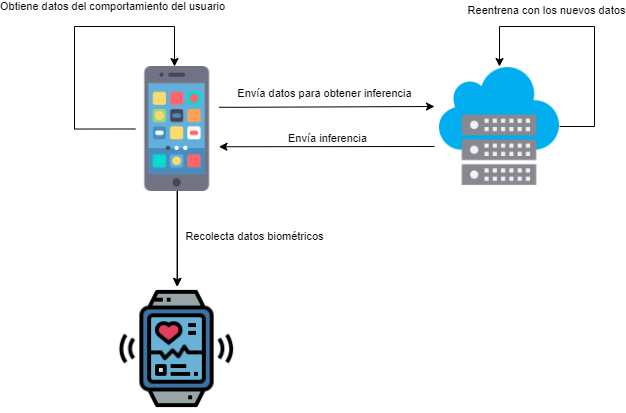
\includegraphics[width=0.66\textwidth]{figures/inception-deck/Componentes.png}
                    \caption{Componentes básicos del sistema}
                    \label{fig:dev:componentes}
                \end{figure}
                
                \vspace*{5mm}
                \begin{figure}[H]
                    \centering
                    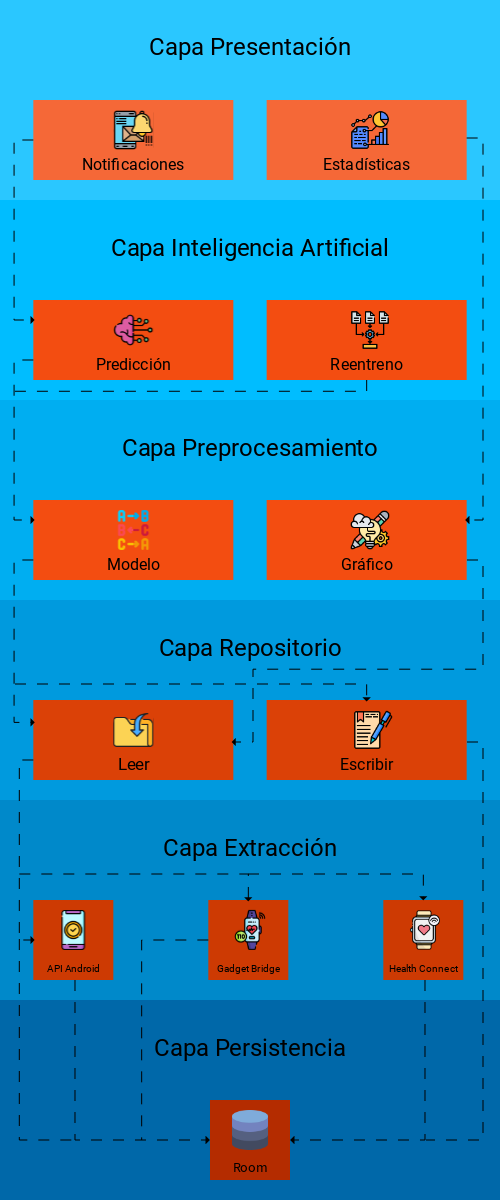
\includegraphics[width=0.475\textwidth]{figures/inception-deck/Pila.png}
                    \caption{Pila con la arquitectura del sistema}
                    \label{fig:dev:arquitecturaPila}
                \end{figure}
            
            \subsubsection{Up at night}
                
                \vspace*{5mm}
                \begin{tabularx}{\textwidth}{ | X | X | }
                    \hline
                    Riesgos en los que podemos influir & Riesgos en los que no podemos influir \\
                    \hline
                        \textbullet\ Realización de pruebas exhaustivas tanto del \textit{backend} como de la interfaz gráfica de usuario.
                        & 
                        \textbullet\ Problemas de compatibilidad entre las versiones de Android.	 \\
                        
                        \textbullet\ Participación de voluntarios que aporten datos al estudio con los que mejorar la precisión y evitar sesgos.
                        &
                        \textbullet\ Muestra de estudiantes variada y contrastada participando en el proyecto. \\
                        
                        \textbullet\ Elaboración de unos términos y condiciones legales acerca de los datos obtenidos en el proyecto.
                        & 
                        \textbullet\ Soportes de los fabricantes de \textit{wearables} (en especial Samsung) a Health Connect. \\
                        
                        \textbullet\ Accesibilidad correcta de la aplicación. 
                        & 
                        \textbullet\ Funcionamiento de las pulseras Xiaomi en aplicaciones no oficiales. \\
                        
                        \textbullet\ Elaboración de un diseño coherente a nivel UX/UI de la aplicación. 
                        & 
                        \textbullet\ Disponibilidad de los datos del móvil y de los \textit{wearables}. \\
                        
                        \textbullet\ Comunicación y difusión eficaz del proyecto en la escuela, en la defensa de este TFM y en redes sociales. 
                        & 
                        \textbullet\ Fiabilidad suficiente de los datos obtenidos por el móvil y los \textit{wearables}. \\
                        
                        \textbullet\ Continuidad del proyecto después del presente TFM para, entre otros, publicar una aplicación en iOS.
                        &
                        \textbullet\ Incumplimiento de la planificación por circunstancias ajenas al proyecto. \\
                        
                        \textbullet\ Definición clara de la arquitectura y de los procesos de mantenimiento y ampliación de la aplicación.
                        &
                        \textbullet\ Retrasos en la entrega del hardware necesario para el sistema. \\
                        
                        
                        \textbullet\ Mantenimiento futuro de la aplicación con las nuevas versiones de Android. 
                        & 
                        \textbullet\ Ausencia de fallos al publicar la aplicación en la Google Play Store. \\
                    
                        
                        \textbullet\ Potencia de cómputo suficiente para entrenar el modelo de Inteligencia Artificial
                        & 
                        \textbullet\ Precisión insuficiente del modelo de Inteligencia Artificial para ser utilizado en un entorno real.\\


                    \hline
                    
                    \caption{Riesgos del proyecto}
                    \label{tab:dev:riesgos}
                \end{tabularx}
                
            \subsubsection{Size it up}
                %begin{landscape}
                \vspace*{5mm}
                \begin{figure}[H]
                    \centering
                    %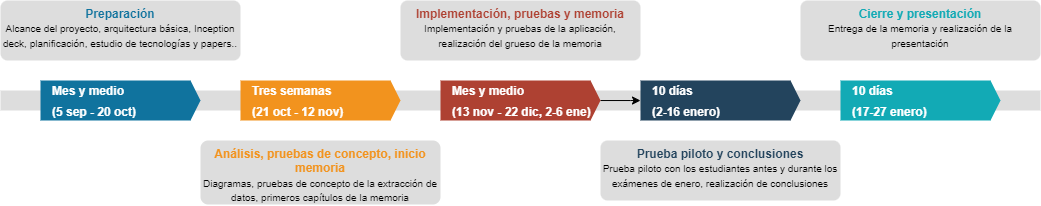
\includegraphics[width=\textheight,angle=90,origin=c]{figures/inception-deck/Size up.png}
                    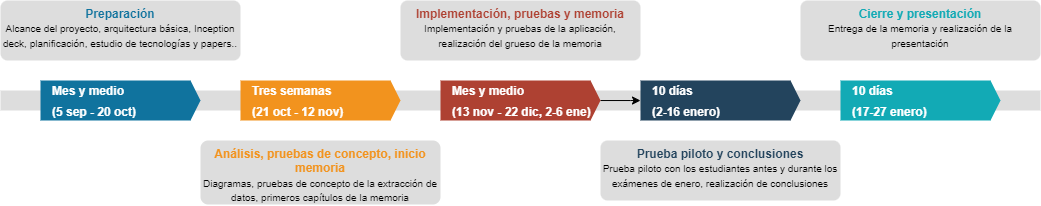
\includegraphics[width=\textwidth]{figures/inception-deck/Size up.png}
                    \caption{Dimensionamiento aproximado del proyecto}
                    \label{fig:dev:sizeItUp}
                \end{figure}
                %\end{landscape}
            \subsubsection{What's going to give}
                
                \vspace*{5mm}
                \begin{tabularx}{\textwidth}{ | >{\hsize=.34\hsize}X | >{\hsize=.14\hsize}X | >{\hsize=.52\hsize} X | }
                    \hline
                        Aspecto 
                        & 
                        Importancia  
                        & 
                        Implicaciones \\
                    \hline
                        Detalle de la documentación
                        & 
                        Media  
                        & 
                        Se desea que la memoria explique detalladamente las cuestiones importantes del proyecto y cubra todo lo realizado en el mismo, pero no es necesario en detalles menores ni se pretende que la memoria sea excesivamente larga. \\
                    \hline
                        Alcance de la implementación 
                        & 
                        Baja - media  
                        & 
                        Una vez realizada la conexión con las API de Android y con el hardware concedido, se puede establecer flexibilidad con el alcance del prototipo. \\
                    \hline
                        Calidad 
                        & 
                        Media - alta  
                        & 
                        Se deben realizar pruebas detalladas y obtener métricas de calidad del software implementado, pero se permite cierta flexibilidad en las mismas sobre el software que maneje el hardware del proyecto por su alta dificultad. \\
                    \hline
                        Comunicación del proyecto 
                        & 
                        Alta  
                        & 
                        Se necesitan usuarios para la prueba piloto y para obtener retroalimentación del proyecto. No obstante, si bien se desea que el proyecto sea continuado, no es estrictamente necesario.\\
                    \hline
                        Experiencia de usuario 
                        & 
                        Media  
                        & 
                        La aplicación debe ser intuitiva y accesible para el usuario, pero no se necesita que el prototipo tenga un diseño visual (elementos, animaciones, gráficas) muy elaborado y detallado al ser un prototipo. \\
                    \hline
                        Fiabilidad 
                        & 
                        Media  
                        & 
                        No están previstas pruebas exhaustivas con todos los dispositivos compatibles (versiones del SO, dispositivos hardware), por lo que \textit{bugs} leves son admisibles. \\
                    \hline
                        Presupuesto (hardware) 
                        & 
                        Muy alta  
                        & 
                        El presupuesto está cerrado al aprobado, por lo que no se pueden incorporar nuevos componentes. \\
                    \hline
                        Rendimiento 
                        & 
                        Baja - media  
                        & 
                        La optimización del software queda fuera del proyecto, si bien se debe de garantizar un rendimiento mínimo para no afectar la experiencia de usuario. \\
                    \hline
                        Seguridad 
                        & 
                        Alta  
                        & 
                        Si bien los datos del móvil no son personales, los de los \textit{wearables} sí lo son, por lo que deben ser debidamente protegidos tanto en su almacenamiento como en su trasmisión con técnicas estándar. \\
                    \hline
                        Tiempo 
                        & 
                        Muy alta  
                        & 
                        El máster proporciona dos convocatorias fijas en el calendario, y por la situación personal del autor solo puede acudir a la de enero, por lo que el proyecto debe finalizar para esa fecha. \\
                    \hline
                    
                    \caption{Cuestiones y prioridades del proyecto}
                    \label{tab:dev:prioridades}
                \end{tabularx}
            
            
            \subsubsection{What it's going to take}
            
                En el apartado de Tómale las medidas se establecieron las etapas del proyecto, por lo que ya conocemos el tiempo estimado de desarrollo del proyecto: cuatro meses y medio. Asimismo, al ser un Trabajo Final de Máster realizado por una persona se necesita a un único ingeniero para el proyecto.
                
                Durante ese plazo las labores del desarrollador incluyen (pero no se limitan a):
                \begin{itemize}
                    \item Análisis y planteamiento del problema a resolver.
                    \item Diseño de un sistema que combine hardware y software.
                    \item Implementación de una aplicación Android con el lenguaje de programación Kotlin.
                    \item Diseño de interfaces de usuario y experiencia de usuario. 
                    \item Comunicación de smartphones Android con dispositivos \textit{wearables} mediante Bluetooth.
                    \item Realización de pruebas unitarias, funcionales y de integración.
                    \item Uso de sistemas de control de versiones, como Github.
                    \item Desarrollo de un pipeline CI/CD.
                    \item Aplicación de metodologías ágiles.
                \end{itemize}
                
                No obstante, son labores que puede desarrollar un perfil con formación universitaria en Informática, ya que al ser un proyecto relativamente breve no se necesita de personal especializado en análisis, pruebas, etc. 
                
                Por tanto, se supone que dicho perfil es un Android Developer y que su salario es el promedio. Según la conocida web de empleo Glassdoor, dicho salario medio en Madrid es de 33.000 €/año, por lo que su salario prorrateado es de 12.375€. Asimismo, hay que sumar el presupuesto concedido por la universidad, que asciende a 460€.
                
                Por tanto, la estimación del coste total del proyecto es de 12.835€.

     
    \section{Setup del proyecto}

    \section{Implementación de la aplicación móvil}

    \section{Implementación de la API del servidor}

        \subsection{Subida de datos de usuario}

        \subsection{Subida de los datos de los cuestionarios}

        \subsection{Datos de la comunidad}
\chapter{[En curso] Pruebas del sistema}
\label{chapter:pruebas}
\chapquote{Las palabras tienen poder, pero sólo si la gente las escucha. Cuando no lo hacen, las acciones hablan lo suficientemente alto como para que cualquiera las escuche.}{Ryosuke Takahashi}
    \section{Aplicación móvil}
    \section{API del servidor}

A diferencia de la aplicación móvil, en esta parte si ha sido posible realizar pruebas automatizadas, siendo una parte importante dentro del \textit{pipeline} CI/CD incorporado en GitHub. 

---
Tenemos
\begin{itemize}
    \item Pruebas con unittest
    \item Coverage de código
    \item Flake como linter para cumplir con PEP8. Complejidad ciclomática de 10.
    \item Mongo db mockeado
\end{itemize}
--
    
        \subsection{Pruebas unitarias}
        \subsection{Pruebas de integración}

\chapter{[En curso] Resultados}
\label{chapter:resultados}

\chapquote{¡Los números Mason! ¿Qué significan?}{Jason Hudson}

\section{Preparación del entorno}
En este apartado se enumeran los pasos seguidos para la preparación del entorno que ha sido utilizado en el desarrollo del sistema.

\subsection{Sistema Operativo}


\subsection{Tecnologia 1}
\subsection{Tecnologia ...}
\subsection{Tecnologia N}

Section{Implementación del caso de estudio} \label{Implementación del caso de estudio}


\section{Resultados del caso de estudio}

En este apartado se muestran algunos ejemplos de los utilización y resultados que podrían obtenerse.

\section{Problemas encontrados}

A continuación se van a detallar todos los problemas encontrados durante el desarrollo
de este Trabajo de Fin de Máster.

\begin{enumerate}
    \item Falta de experiencia del menda en apps móviles, proceso de aprendizaje
    \item Soporte de los fabricantes fuera de Fitbit, Samsung y de mala gana
    \item Madurez en Jetpack Compose y especialmente en Material Design 3
    \item Cambios de Health Connect al estar en testeo
    \item Cosas más avanzadas en vico
    \item Manejo de parámetros en las ventanas
    \item Componentes gráficos que no estaban, como el progreso circular
    \item Diseñar una arquitectura a nivel de implementación que soportarse tantas combinaciones posibles, como cuestionarios numericos y no numericos, el caso especial de suicido que se cierra antes de llegar al final...
    \item Gráficas en Android en general, y más siendo responsives
    \item Poco soporte en Android para elegir manualmente el idioma
    
    \item Dificultades para testeo
    \item Implementaciones diferentes según móvil, especialmente work manager
    
\end{enumerate}
\chapter{[Por revisar] Impacto social y medioambiental}
\label{chapter:aspectos}

\chapquote{Si tienes tanto miedo al fracaso, nunca tendrás éxito.}{Mario Andretti}

En este capítulo se recogen los beneficios que la implantación del proyecto desarrollado podría generar tanto a nivel social como medioambiental.

\section{Aspectos éticos, sociales y económicos}
    El sistema propuesto tiene un impacto considerable en estas cuestiones, al buscar contribuir en la mejora de la salud mental de las personas. En primer lugar, se puede observar el impacto de este proyecto en base a los \gls{ods} respecto a los siguientes objetivos globales:

    \begin{itemize}
        \item \textbf{Salud y bienestar}: el sistema contribuye claramente a la visibilización y concienciación acerca de la salud mental, a través de la detección de trastornos en personas que posiblemente lo desconozcan y comunicando recomendaciones para evitar en la medida que dichos trastornos se agraven\footnote{Recordar una vez más que el sistema no pretende desplazar a los profesionales de la psicología, sino ser un apoyo para los mismos. En casos graves la solución pasa necesariamente por especialistas.}. No obstante, este tipo de iniciativas deben ir acompañadas de políticas públicas que permitan resolver cuestiones como las listas de espera o de la ausencia de profesionales, ya que un diagnóstico precoz de un trastorno grave es poco útil si no va acompañado de un tratamiento de calidad por parte de profesionales.
        \item \textbf{Educación de calidad}: al proporcionar consejos y pautas avaladas por profesionales de la psicología, los usuarios pueden acceder a información respaldada científicamente; la cual puede mejorar su calidad de vida. No obstante, como se mencionó en el punto anterior, estos consejos son una parte de la solución a estos problemas, pero no pueden resolverlos por sí solos.
        \item \textbf{Reducción de las desigualdades}: como se vió en la Sección \ref{sec:justificacion}, existen numerosas desigualdades en el acceso a la atención psicolópgica. En este ámbito, los requisitos técnicos del sistema son alcanzables por \glspl{smartphone} baratos, facilitando el acceso a la información psicológica independientemente del contexto socio-económico.
        \item \textbf{Producción y consumo responsable}: el sistema no requiere hardware específico, limitándose a hacer uso de los recursos que disponga el usuario. Asimismo, el sistema no marca restricciones adicionales a las ya impuestas por sus dependencias, evitando en general promover el consumo nuevos productos.
    \end{itemize}

    En cuanto a las cuestiones de privacidad, cabe destacar que el uso de componentes como \textit{Salud Conectada} y el uso de un servidor de la \gls{etsisi}. Estas circunstancias permiten mejorar la privacidad de los usuarios frente a otras soluciones como \textit{Google Fit}, ya que los datos únicamente están o bien en el dispositivo del usuario o anonimizados dentro de la Escuela. 
    
    Con esto se logra evitar el trasvase de información a servidores alojados en países fuera de la Unión Europea, donde las normativas de protección de datos son más laxas; como es el caso de los Estados Unidos. 

    Por otra parte, a nivel ético existen numerosas preocupaciones en el ámbito de las \gls{tic}, ya que las prácticas deshonestas expuestas en la Sección \ref{sec:estado_arte:apps} no se limitan a las aplicaciones de salud mental.
    
    Algunas plataformas digitales muy conocidas están diseñadas específicamente para explotar ciertos resortes psicológicos del ser humano. Redes sociales como \textit{Instagram} o \textit{TikTok} utilizan fenómenos como la gratificación instantánea o los mecanismos de recompensa \cite{noauthor_dopamina_2022} para espolear la liberación de dopamina\footnote{Se trata de un neurotransmisor asociado con funciones cerebrales, tales como la motivación, el aprendizaje y la recompensa, entre otras \cite{gil_que_2023}.}, pudiendo provocar desde la adicción a las mismas redes, hasta problemas de ansiedad o de autoestima cuando no se reciben dichas recompensas \cite{ina_impacto_2023}.
    
    Por otra parte, este mecanismo de gratificación instantánea también es explotado por algunos videojuegos a través de las \textit{lootboxes} (o \textit{cajas botín} en castellano), las cuales provocan grandes réditos económicos al provocar graves problemas de adicción, especialmente entre los menores. Debido a este contexto, las instituciones están tomando medidas para limitar técnicas como el \textit{scroll infinito} \cite{alconchel_prohibir_2023} o de limitar el acceso a las \textit{lootboxes} \cite{ministerio_de_derechos_sociales_consumo_y_agenda_2030_ministerio_2024} \cite{garcia_espanda_2024}. 
    
    En este marco cabe recalcar la apuesta firme de este proyecto por la psicología que permita ayudar a las personas a afrontar sus problemas de salud mental, sin fines ocultos o funcionalidades perversas. Como ya se reflejó a lo largo de este documento, la transparencia y la privacidad de los usuarios son baluartes fundamentales de esta iniciativa.

\section{Contexto medioambiental}

    Antes de comenzar con esta sección, cabe destacar que este proyecto no está diseñado para interactuar directamente con el medioambiente, por lo que el impacto del mismo en el entorno se puede considerar como indirecto.

    Al tratarse de un sistema que busca ante todo un diagnóstico precoz de las enfermedades de salud mental, existen potenciales beneficios en esa línea. De finalizarse este prototipo e implementarse en la comunidad universitaria, podrían detectarse estos estos trastornos en etapas más tempranas, lo cual podría reducir la gravedad de los mismos, redundando en tratamientos médicos más cortos.

    Para lograr este cometido, el sistema necesita realizar una serie de tareas, las cuales tienen cierto impacto en el medio ambiente. Una de estas actuaciones es la extracción de datos de los \glspl{wearable}. El sistema propuesto únicamente consume, de existir, los datos ya leídos por el fabricante del dispositivo; los cuales se alojan únicamente en el dispositivo del usuario. Por tanto, el impacto de estas lecturas es muy pequeño, ya que no se obliga al usuario a comprar un \gls{wearable} ni se realiza comunicación redudante con el aparato.

    Por otra parte, en cuanto a la comunicación con el servidor, al utilizarse un servidor de la \gls{etsisi}, el envío de los datos a través de la red es relativamente ligero. Asimismo, en la implementación se realizaron una serie de optimizaciones para enviar únicamente los datos necesarios cada 8 horas; por lo que no se trata de un sistema que realice un elevado consumo de la red y de energía.

    No obstante, el principal escollo en cuanto al medio ambiente sería la adición de un modelo para mejorar sensiblemente la detección de los niveles de salud mental; que si bien está fuera de la implementación actual, su incoporación futura podría ser muy útil. 
    
    La popularización de modelos de Inteligencia Artificial, como \textit{ChatGPT}, ha provocado que hasta la \gls{iea} haya convocado una conferencia sobre este tema \cite{perez_demanda_2024}, ya que se estima que el consumo de energía de los centros de datos oscile entre el 3 y el 4\% del consumo global \cite{gijon_inteligencia_2024}; mientras que para 2027, el consumo de electricidad de estos sistemas a nivel mundial podría aumentar entre 85 y 134 TWh anuales, cantidad comparable al consumo anual de electricidad de países como los Países Bajos, Argentina y Suecia \cite{redaccion_inteligencia_2023}.
    
    En ese sentido, para paliar el potencial impacto medioambiental se podría continuar con el enfoque de localizar estos servidores en la \gls{etsisi}; y apostar por el uso de energías limpias, como la solar; para alinearse con los \gls{ods} y en particular, con el número 7: \textit{Energía asequible y no contaminante}. El objetivo de estos movimientos sería reducir el consumo energético en la medida de lo posible, y basar ese consumo en fuentes de energía que tengan un impacto lo más reducido posible en el medioambiente.
\chapter{Presupuesto}
\label{chapter:presupuesto}

\chapquote{Lo perfecto es enemigo de lo bueno.}{Cita atribuida a Voltaire}
\chapter{[En curso] Conclusiones y líneas futuras}
\label{chapter:conclusiones}

\chapquote{Realiza cada una de tus acciones como si fuera la última de tu vida.}{Marco Aurelio}

\section{Conclusiones}

Suelen poner 2 caras, si nos ponemos bravos tira a 4

\section{Lineas futuras}
    \label{section:lineas_futuras}
    
    En primer lugar, el trabajo futuro más prioritario es la implementación de los requisitos que no han sido cubiertos en este primer desarrollo. Dichos requisitos, junto con sus líneas de actuación propuestas, son:

    \begin{itemize}
        \item \ref{req:no_funcionales:datos_solo_cientificos} \textit{El acceso a los datos anonimizados de los usuarios solo estará permitido para propósitos científicos.}
        
        Para ello se necesita definir una política de acceso a los datos, la cual debe aceptarse por los analistas de datos. En este aspecto es recomendable contar con asesoría legal.
        Posteriormente se debería diseñar e implementar un sistema de acceso que permita la administración de los diferentes usuarios.
        
        \item \ref{req:no_funcionales:ddos} \textit{El servidor que aloje los datos anonimizados deberá estar protegido antes ataques de denegación de servicio y accesos no autorizados.}

        Para cumplir con este requisito, se deberá definir e implementar un conjunto de medidas que permitan proteger a dicho servidor, en consonancia con los recursos disponibles en la \gls{etsisi}.
        
        \item \ref{req:no_funcionales:cifrado_comunicaciones} \textit{Las comunicaciones entre aplicación y servidor deberán estar cifradas.}

        La implementación de este requisito consta de las siguientes fases:
        \begin{enumerate}
            \item Generar un certificado \gls{ssl} por parte de una autoridad de certificación reconocida.
            \item Modificar la \gls{api} para usar \gls{https} con el certificado anterior.
            \item Restringir la aplicación para que únicamente acepte conexiones \gls{https}.
        \end{enumerate}
        
        \item \ref{req:no_funcionales:politica_privacidad} \textit{Se deberá definir una política de privacidad de acuerdo al \gls{rgpd} \cite{publications_office_of_the_european_union_reglamento_nodate} y a las directrices de \textit{Salud Conectada} \cite{google_preguntas_nodate}.}

        Se recomienda nuevamente contar con asesoría legal para la conformidad de dicha política. Por otra parte, dicha política debe ser accesible desde fuera de la aplicación, para garantizar que los usuarios puedan leerla antes de comenzar el uso o descarga de la aplicación. 
    \end{itemize}

    Una vez todos los requisitos planteados hayan sido satisfechos, se podría desplegar la aplicación en tiendas virtuales como \textit{Play Store}, dotando al proyecto de mucho mayor alcance y de una retroalimentación mucho más amplia y profuda.
    
    Asimismo, otra línea de trabajo propuesta es la realización de ciertas mejoras en el marco de los requisitos de usuario ya implementados. En el caso de los requisitos de seguimiento (\ref{req:usuario:seguimiento_estres}, \ref{req:usuario:seguimiento_depresion}, \ref{req:usuario:seguimiento_soledad} y \ref{req:usuario:seguimiento_suicidio}), la principal mejora sería la incorporación de un modelo basado en Inteligencia Artificial que permita mejorar el diagnóstico precoz. 
    
    Para ello se podría realizar un estudio científico que explore esta posibilidad en el que se recojan datos de los usuarios, algo que ya permite el estado actual del proyecto. Este estudio podría experimentar con los datos recogidos y/o con los datos de los estudios detallados en las Secciones \ref{sec:estado_arte:biometricos} y \ref{sec:estado_arte:smartphone}. Asimismo, la arquitectura planteada permite un despliegue sencillo, con el cual se podría evaluar la eficacia del mismo.

    En cuanto a los requisitos de consejos (\ref{req:usuario:consejo_estres}, \ref{req:usuario:consejo_depresion}, \ref{req:usuario:consejo_soledad} y \ref{req:usuario:consejo_suicidio}) se anima al resto de estudiantes y a la \gls{etsisi} a ahondar en la colaboración con profesionales de la Psicología para la elaboración de nuevas pautas. El estado actual del proyecto permite a dichos profesionales desplegarlos con muy poco coste, por lo que se podrían realizar trabajos de investigación que exploren el impacto de dichos consejos.

    Finalmente, se enumeran otras líneas de trabajo que son factibles de realizar a largo
    plazo para ampliar y refinar el proyecto:
    
    \begin{enumerate}
        \item Elaboración de un conjunto de pruebas automáticas exahustivas para la aplicación móvil, incluyendo reportes de \textit{coverage} del código.
        \item Comprobar la recolección de datos en otras pulseras, tanto de Fitbit como de otros fabricantes.
        \item Realizar agregación de datos para ciertas variables, como las pulsaciones, para aligerar el volumen de datos.
        \item Explorar cuestiones relacionadas con la infraestructura, como el despliegue de la funcionalidad del servidor mediante contenedores, lo que permitiría una mejor escalabilidad del mismo.
        \item Segmentar la comunidad de usuarios para mejorar la representatividad del conjunto.
        \item Estudiar la imputación de datos nulos con otras técnicas, tales como: regresión, \textit{Last Observation 
        Carried Forward}, \textit{Next Observation Carried Backward}... \cite{gupta_null_nodate}
        \item Añadir \textit{features} relacionadas con los cuestionarios puntuales: gráficas, notificaciones...
        \item Diseñar e implementar una interfaz gráfica centrada en las pantallas \textit{expandidas}\footnote{Pantallas 
        que disponen de más de 840dp de ancho o 900dp de alto}.
        \item Localizar la aplicación a más idiomas.
    \end{enumerate}

\chapter{Líneas futuras}
\label{chapter:lineas}

\chapquote{La victoria más bella es siempre la próxima.}{Enzo Ferrari}

\todo[inline]{Comprobar si hemos hablado del sistema como prototipo}

Al ser el sistema de este proyecto un prototipo, existen numerosas vías para ampliarlo y refinarlo. Algunas de dichas
mejoras son:

\begin{enumerate}
    \item Cifrado de las comunicaciones entre la app y el servidor mediante un certificado SSL en el propio servidor.
    \item Establecimiento de una política de privacidad detallada. Este punto es imprescindibile para poder publicar la
    aplicación (en tiendas virtuales como Play Store) y recoger datos con legalidad.
    \item Desplegar la aplicación en el ámbito universitario. Realizándolo se podría obtener una retroalimentación más
    amplia y profunda de la aplicación, y además se podrían recolectar datos para entrenar
    modelos que predigan cada una de las variables de Salud Mental.
    \item Comprobar la recolección de datos en otras pulseras, tanto de Fitbit como de otros fabricantes.
    \item Adaptar la aplicación para soportar Android 14. Como hemos comentado en la sección 
    \ref{section:salud_conectada}, Android 14 vendrá preinstalado, y Google ha decidido introducir cambios notables, 
    pasando Salud Conectada de ser un APK a un \textit{framework} \cite{noauthor_como_nodate-1}, por lo que se necesita
    ajustar la aplicación para cubrir este caso.
    \item Elaboración de un conjunto de pruebas exahustivo para la aplicación móvil, incluyendo reportes de 
    \textit{coverage} del código.
    \item Establecer que al instalar la aplicación se realice un cuestionario diario. Según la hora del día se elegiría
    si realizar el de mañana o el de noche, pero en cualquier momento del día uno de esos dos.
    \item Dar más presencia a los cuestionarios puntuales, ya sea con gráficas, notificaciones...
    \item Estudiar la imputación de datos nulos con otras técnicas, tales como: regresión, \textit{Last Observation 
    Carried Forward}, \textit{Next Observation Carried Backward}... \cite{gupta_null_nodate}
    \item Realizar agregación de datos para ciertas variables, como las pulsaciones, para aligerar el volumen de datos.
    \item Diseñar e implementar una interfaz gráfica centrada en las pantallas \textit{expandidas}\footnote{Pantallas 
    que disponen de más de 840dp de ancho o 900dp de alto}.
    \item Localizar la aplicación a más idiomas.
    \item Disponer de al menos dos pautas de recomendación a los usuarios para cada variable y estado.
    \item Segmentar la comunidad de usuarios para mejorar la representatividad del conjunto.
\end{enumerate}

\chapter{Temporal}
%\chapter{Referencias, glosarios e índices}
\label{ch:referencias}

En este capítulo mostraremos cómo crear nuevas referencias bibliográficas, entradas en el glosario de términos y acrónimos y palabras para el índice.

\section{Referencias bibliográficas}
\label{s:referencias-bibliograficas}

Hay muchas formas diferentes de gestionar las referencias bibliográficas, así que aquí hemos decidido elegir una de ellas por considerarla la más cómoda y simple, que es mediante el paquete \textit{biblatex}.

El fichero de referencias, \texttt{references.bib}, incluirá una entrada por cada una de las referencias que se citan durante la memoria. Luego, en el cuerpo del texto, se podrán hacer referencias a dichas entradas y será \LaTeX~después quien se encargue de indexar correctamente, crear los hipervínculos y maquetar automáticamente.

El fichero \texttt{references.bib} puede tener muchas más de las referencias que se citan en el cuerpo del texto. Sin embargo, sólo aparecerán las referencias que se citen en el texto.

\notebox{\textbf{No has dicho en ningún momento \textit{bibliografía}} Sí. Las referencias bibliográficas, también conocidas como lista de referencias o simplemente referencias, son todas aquellas fuentes bibliográficas que han sido citadas a lo largo del documento. La bibliografía, también conocida como referencias externas, es simplemente una lista de recursos utilizados, citados o no. Como generalmente los no referenciados no se usan para dar soporte a un texto científico se suelen descartar.}
 
\subsection{¿Cómo creamos nuevas referencias?}

El fichero \texttt{references.bib} contará cero o más entradas con la estructura mostrada en el listado~\ref{lst:base-bibref}.

\begin{lstlisting}[language=tex,caption=Estructura general de una referencia]
@tipo{id,
    author = "Autor",
    title = "Título de la referencia (libro, artículo, enlace, ...)",
    campo1 = "valor",
    campo2 = "valor",
    \ldots
}
\end{lstlisting}

En esta entrada, \texttt{@tipo} indica el tipo de elemento (p. ej. \texttt{@article} para artículos o \texttt{@book} para libros) e \texttt{id} es un identificador \textbf{único en todo el documento} para el elemento. El resto de campos dependerán del tipo de la referencia, aunque generalmente casi todos los tipos comparten los campos de \texttt{author}, \texttt{title} o \texttt{year}.

AQUÍ CONTAR CÓMO SE AÑADEN ENTRADAS, LAS POSIBLES OPCIONES Y EL ENLACE A DONDE SE DESCRIBE TODO EN PROFUNDIDAD

\subsection{¿De qué manera puedo citar las referencias?}

AQUÍ CONTAR LAS DIFERENTES OPCIONES PARA REFERENCIAR ARTÍCULOS. PONGO LA BÁSICA, QUE ES~\cite{mcculloch1943logical}, PARA QUE ME APAREZCA EL CAPÍTULO DE REFERENCIAS.

\section{Referencias cruzadas}

\section{Referencias a recursos externos}

\section{Glosario y acrónimos}
\label{s:glosario}
Para gestionar el glosario y los acrónimos se hace uso del paquete \texttt{glossaries}. Es, quizá, algo complejo de configurar ya que permite muchas opciones diferentes.

Aquí proponemos una configuración por defecto para que lo único que haya que hacer sea añadir y referenciar las entradas.

\subsection{Definiendo los términos del glosario}

Un listado aquí todo majo:

\begin{lstlisting}[language=TeX]
\newglossaryentry{ex}{
    name={sample},
    description={an example}
}
\end{lstlisting}

\section{Índice}
%\chapter{Licencia}
\label{ch:licencia}

Cuando se publica la obra en el archivo digital, por defecto lo hace con la licencia de CC Reconocimiento - Sin obra derivada - No comercial. Aunque usar cc guay, esta licencia no es una licencia libre y a algunos nos parece algo malo.

Considero que todo el conocimiento generado en una universidad pública ha de ser público y libre. Por ello, aunque por defecto está puesto ese, recomiendo usar \texttt{\\documentclass\{upm-report\}}, de tal manera que mientras se respete que se comparte igual, todo el mundo puede hacer de esta obra el uso que quiera.

De todas formas, indican que si el autor quiere usar otra licencia de Creative Commons deberá ponerse en contacto con el Administrador del Archivo Digital UPM: archivo.digital@upm.es.

% TODO Poner todas las opciones posibles de licencia y explicarlas

\href{https://www.google.com}{Google}


\printbibliography

\appendix
\chapter{Cuestionarios para el seguimiento diario}
\label{chapter:cuestionarios}
    \section{Inicio del día}
        \subsection{Estrés}
            \begin{enumerate}
                \item Me siento nervioso/a
                \item Me siento angustiado/a
                \item Me siento activo/a
                \item Estoy preocupado/a
            \end{enumerate}
            La respuesta a cada pregunta es un número entero en la escala de 0 a 10.

        \subsection{Depresión}
            \begin{enumerate}
                \item Me siento triste
                \item Me siento vacío/a 
                \item Me siento apático/a
            \end{enumerate}
            La respuesta a cada pregunta es un número entero en la escala de 0 a 10.

        \subsection{Soledad}
            \begin{enumerate}
                \item Me siento solo/a
                \item Me siento incomprendido/a
                \item Me siento exclusivo/a
                \item Me siento poco ayudado/a
            \end{enumerate}
            La respuesta a cada pregunta es un número entero en la escala de 0 a 10.

        \subsection{Suicidio}
            \begin{enumerate}
                \item Tengo pensamientos de suicidio
                \item En los últimos días, ¿has pensado seriamente en suicidarte?
                \item ¿Existe alguna posibilidad de que pienses acabar con tu vida hoy o en los próximos días?
            \end{enumerate}
            Las posibles respuestas a cada pregunta es sí o no.

    \section{Final del día}
        \subsection{Estrés}
            \begin{enumerate}
                \item Me he sentido nervioso/a
                \item Me he sentido angustiado/a
                \item Me he sentido activo/a
                \item He estado preocupado/a
            \end{enumerate}
            La respuesta a cada pregunta es un número entero en la escala de 0 a 10.

        \subsection{Depresión}
            \begin{enumerate}
                \item Me he sentido triste
                \item Me he sentido vacío/a 
                \item Me he sentido apático/a
            \end{enumerate}
            La respuesta a cada pregunta es un número entero en la escala de 0 a 10.

        \subsection{Soledad}
            \begin{enumerate}
                \item Me he sentido solo/a
                \item Me he sentido incomprendido/a
                \item Me he sentido exclusivo/a
                \item Me he sentido poco ayudado/a
            \end{enumerate}
            La respuesta a cada pregunta es un número entero en la escala de 0 a 10.

        \subsection{Suicidio}
            \begin{enumerate}
                \item He tenido pensamientos de suicidio
                \item En el día de hoy, ¿has pensado seriamente en suicidarte?
                \item ¿Existe alguna posibilidad de que pienses acabar con tu vida hoy o en los próximos días?
            \end{enumerate}
            Las posibles respuestas a cada pregunta es sí o no.

        \subsection{Contraste}
            \begin{enumerate}
                \item ¿Has experimentado cambios en el apetito?
                
                Posibles respuestas:
                    \begin{itemize}
                        \item Excesivamente alto  
                        \item Adecuado
                        \item Excesivamente bajo
                    \end{itemize}

                \item ¿Con cuánta energía te has notado?
                
                Posibles respuestas:
                    \begin{itemize}
                        \item Alta
                        \item Moderada
                        \item Baja
                    \end{itemize}

                \item ¿Cuál ha sido tu nivel de descanso?
                
                Posibles respuestas:
                    \begin{itemize}
                        \item Satisfactorio  
                        \item Moderado
                        \item Insuficiente
                    \end{itemize}
                    
                \item Tu nivel de concentración ha sido…
                
                Posibles respuestas:
                    \begin{itemize}
                        \item Satisfactorio  
                        \item Adecuado
                        \item Insuficiente
                    \end{itemize}
                    
                \item ¿Cuál ha sido tu nivel de líbido?
                
                Posibles respuestas:
                    \begin{itemize}
                        \item Satisfactorio  
                        \item Adecuado
                        \item Insuficiente
                    \end{itemize}
                    
                \item ¿Cómo te has encontrado a nivel de dolor?
                
                Posibles respuestas:
                    \begin{itemize}
                        \item Sin dolor 
                        \item Dolor moderado
                        \item Dolor alto
                    \end{itemize}
                    
            \end{enumerate}
\chapter{Recomendaciones}
\label{chapter:recomendaciones}

    \section{Estrés}
        \subsection{Bajo}
            Estupendo, sigue así. 
        \subsection{Moderado}
            \subsubsection{Pauta 1}
                Hemos percibido que estás experimentando niveles moderados de ansiedad o estrés. 
                Por ello, te recomendamos que planifiques un espacio en el día de hoy para hacer ejercicio físico.

                El ejercicio físico puede disminuir el estrés por varias razones:
                \begin{itemize}
                    \item Liberación de endorfinas: Durante el ejercicio, el cuerpo libera endorfinas, que son hormonas que  actúan como analgésicos naturales y generan sensaciones de bienestar. 
                    \item Reducción de la hormona del estrés: El ejercicio regular puede disminuir los niveles de cortisol, la hormona del estrés.
                    \item Mejora del sueño: El ejercicio regular puede promover un sueño más profundo y reparador.
                    \item Distracción y enfoque: Participar en actividades físicas puede distraer la mente de las preocupaciones y tensiones diarias. Cuando te concentras en el ejercicio, tu mente se enfoca en la actividad física en lugar de en los problemas, lo que puede ayudar a reducir el estrés y proporcionar un descanso mental.
                    \item Aumento de la confianza y la autoestima: El ejercicio regular puede ayudar a mejorar la confianza y la autoestima. Al establecer metas y lograr objetivos en el ámbito del ejercicio, puedes desarrollar una mayor sensación de logro y fortaleza personal. Esto puede ayudar a reducir el estrés al 
                    proporcionar una sensación de control y empoderamiento sobre tu vida.
                \end{itemize}

            \subsubsection{Pauta 2}
                En caso de que no dispongas de mucho tiempo, te proponemos una serie de alternativas. 

                \begin{itemize}
                    \item Trata de buscar un momento para ti, libre de estímulos estresantes. Puedes salir a dar un pequeño paseo, darte una ducha relajante, poner música y centrarte en escucharla durante unos minutos, practica unos estiramientos corporales… El objetivo es rebajar de forma rápida los niveles de ansiedad para poder retomar las tareas desde un estado emocional más adecuado. 
                    \item Trata de eliminar algunos estímulos que puedan estar aumentando tu ansiedad: apaga el móvil a partir de determinada hora en la noche para tener unas horas libres de notificaciones antes de dormir, ponte unos cascos con música relajante para no escuchar el ruido de alrededor, si tienes pendiente tomar una decisión o discutir algo con alguien, aplázalo durante unas horas o días y permítete posponer los pensamientos al respecto, etc. El objetivo es eliminar los estímulos que están produciendo estrés para poder rebajar los niveles de ansiedad y así enfrentarnos de forma más adecuada a nuestros problemas o dificultades. 
                \end{itemize}
        \subsection{Alto}
            Te proponemos que realices un ejercicio de respiración abdominal. 

            El objetivo de esta técnica es regular la respiración y, en consecuencia, disminuir la respuesta de activación fisiológica y la sensación de ansiedad. 
            
            Para ello, trata de llevar el aire hasta tu abdomen en cada inspiración para llenar tus pulmones en profundidad. Visualmente, deberías observar cómo tu tripa se hincha al llenarse de aire. Al expulsar el aire durante la espiración, el abdomen debería retornar a su posición habitual. Evita mover el pecho, los hombros o las clavículas, pues esto indica que el aire está llegando únicamente a la parte superior de los pulmones.
            
            Inhala durante la ascensión de la curva y exhala durante el descenso. Trata de no hacerlo de forma demasiado profunda. Puedes repetirte mentalmente una palabra como calma o relax, puedes imaginar que estás en un lugar tranquilo, o centrar tu atención en cómo el aire entra y sale y cómo la tensión se escapa con cada exhalación. 
    
    \section{Depresión}
        \subsection{Baja}
            Estupendo, sigue así. 
        \subsection{Moderada}

            Te proponemos que incluyas en tu  día de hoy alguna actividad agradable o placentera. 
            
            Es posible que sientas que no tienes ganas o energía para hacerlas o, incluso, que aunque las hagas no lo disfrutarás. No obstante, es importante que entiendas que “las ganas se hacen”. 
            
            Esto significa que cuando nuestro estado de ánimo está un poquito bajo, si esperamos a experimentar ganas para hacer las cosas, probablemente nunca las hagamos. Esto a su vez hará que nuestro estado de ánimo disminuya todavía más, y entremos en un circulo vicioso en el que no haremos nada porque no tenemos ganas porque estamos tristes, y como no hacemos nada estaremos aún más tristes. 
            
            Para no caer en esta problemática te sugerimos que realices alguna actividad agradable, que no sea muy costosa y que te permita sentirte mejor. Pueden ser actividades que hagas tú solo/a o acompañado/a. 
            
            Aquí te dejamos algunas sugerencias. 
            \begin{itemize}
                \item Dar un paseo al aire libre. 
                \item Ir a comprar al supermercado y cocinar una receta que te guste. 
                \item Ver una serie o película que te apetezca.
                \item Quedar con un amigo/a tomar algo o pasear.
                \item Leer un libro, escuchar música, dibujar… 
            \end{itemize}

        \subsection{Alta}
            Te sugerimos que busques apoyo en las personas de tu alrededor.

            Es muy beneficioso que puedas expresar cómo te estás sintiendo a otras personas. El mero hecho de contarlo supondrá un desahogo emocional que te hará sentirte mejor.
            
            Además, las personas que te escuchen podrán comprender por lo que estás pasando y mostrar su empatía y apoyo. Es posible también que puedan tratar de ayudarte u ofrecerte consejos.
            
            Para que todo vaya bien, trata de elegir a la persona adecuada en el momento adecuado. Busca a una persona que se encuentre bien, que no esté muy estresada u ocupada, que te haya mostrado su afecto en alguna ocasión…
            
            Si necesitas desahogarte con frecuencia, trata de hacerlo con diferentes personas y no focalizarte solo en una, ya que prestar apoyo emocional en ocasiones puede resultar algo cansado.
           
            Por último, ten cuidado de no caer en la queja: comunica tus emociones tratando de buscar soluciones y formas de sentirte mejor, en lugar de anclarte en el problema que ha sucedido.

    \section{Soledad}
        \subsection{Baja}
            Estupendo, sigue así. 
        \subsection{Moderada}
            Te sugerimos que busques apoyo en las personas de tu alrededor.

            Es posible que consideres que no tienes a nadie con quién hablar. Sin embargo, si lo intentas, seguro que puedes encontrar personas deseosas de conversar contigo.
            
            Busca a tu alrededor: un vecino con quien hayas tenido contacto, el camarero del bar o el restaurante al que vas en ocasiones, un compañero de trabajo…Puedes tratar de entablar una conversación preguntándoles cómo se encuentran y comentando cosas sobre el ambiente (el tiempo, los precios, los horarios, etc.).
            
            Después, puedes intentar contar alguna anécdota o experiencia personal reciente. Por ejemplo, un programa de TV que te haya gustado, algo curioso que hayas visto recientemente en redes sociales, un plan al que tengas ganas de asistir o que hayas disfrutado si ya lo has hecho, etc.
           
            Poco a poco, podrás progresar en la conversación y hablar más a menudo con estas personas.

        \subsection{Alta}
            Te recomendamos que llames a Cruz Roja Te Escucha (900 107 917).

            Cruz Roja te escucha es una iniciativa que trata de ofrecer acompañamiento y apoyo a personas que se encuentran en una situación de soledad no deseada. 
            
            Podrán facilitarte pautas para sentirte mejor y ofrecerte recursos en tu localidad que puedan servirte de apoyo. 
            
            Puedes contactar en el 900 107 917, de lunes a jueves laborales de 10h a 14h y de 16h a 20h (una hora menos en Canarias) y los viernes laborables de 10 a 14h (una hora menos en Canarias). La llamada es gratuita y confidencial.
    
    \section{Riesgo de suicidio}
        \subsection{Bajo}
            Estupendo, sigue así. 
        \subsection{Moderado}
            Recuerda que, si en algún momento tienes pensamientos relacionados con el suicidio, es importante que pidas ayuda.

        \subsection{Alto}
            Por lo que nos has contado, creemos que el riesgo de que puedas hacerte daño o de que acabes con tu vida es alto.

            Por favor, acude cuanto antes a un servicio de emergencias o llama a los teléfonos 112 o 024. 
            
            Allí encontrarás personas que podrán comprender cómo te sientes y ayudarte a sentirte mejor. 
            
            Recuerda que el suicidio es la única opción que no tiene vuelta atrás. Trata de agotar otras posibles soluciones y pide ayuda para conseguirlo.
%\chapter{Código fuente del proyecto}
\label{chapter:codigo}
% \chapter{Escuelas y títulos}
\label{ch:escuelas-y-titulos}

A continuación se describen todas las opciones de grados y títulos disponibles en la memoria.

\section{Escuelas}

Las escuelas disponibles se describen en el cuadro~\ref{tbl:schools}.

\begin{table}[h]
    \centering
    \begin{tabular}{@{}ll@{}}
        \toprule
        \textbf{Clave}  & \textbf{Valor} \\
        \midrule
        \texttt{etsii}  & E.T.S. de Ingenieros Industriales \\
        \texttt{etsisi} & E.T.S. de Ingeniería de Sistemas Informáticos \\
        \bottomrule
    \end{tabular}
    \caption{\label{tbl:schools} Relación entre el código de la plantilla y la escuela a la que se refiere}
\end{table}

De momento no están todas, así que si te apetece añadir la tuya puedes, o bien contactar con los autores, o bien modificarlo (mira el apéndice~\ref{ch:ampliar}) y también contactar con los autores, así lo podemos hacer público con la mayor cantidad de usuarios posible.

\section{Titulaciones}

RELLENAR; FALTAN, ADEMÁS DE TITULACIONES DE OTRAS ESCUELAS, LOS MÁSTERS Y LOS PROGRAMAS DE DOCTORADO

ETSII: Grados: 05TI (Grado en Ingeniería en Tecnologías), 05IQ (Grado en Ingeniería Química), 05IR (Grado en Ingeniería de Organización) y 05IE (Grado en Ingeniería de la Energía)
ETSISI: Grados: 61CDIA (Grado en Ciencia de Datos e Inteligencia Artificial), 61CI (Grado en Ingeniería de Computadores), 61IW (Grado en Ingeniería del Software), 61SI (Grado en Sistemas de Información), 61TI (Grado en Tecnologías para la Sociedad de la Información)
ETSISI: Másters: 61MSSDE (Máster en Desarrollo Software de Sistemas Distribuidos y Empotrados)

%{\Huge\underline{\colorbox{blue!30}{\textit{\textbf{\textcolor{red}{c}\textcolor{blue}{l}\textcolor{green}{i}\textcolor{pink}{e}\textcolor{purple}{n}\textcolor{yellow}{t}\textcolor{orange}{e}}}}}}%

% \chapter{¿Cómo ampliar la plantilla?}
\label{ch:ampliar}
% \chapter{Lista de paquetes incluidos}
\label{ch:paquetes}

\printglossary

\end{document}
